%%%%%%%%%%%%%%%%%%%%%%%%%%%%%%%%%%%%%%%%%%%%%%%%%%
% Basic setup. Most papers should leave these options alone.
\documentclass[a4paper,fleqn,usenatbib,useAMS,usedcolumn]{mnras}

% MNRAS is set in Times font. If you don't have this installed (most LaTeX
% installations will be fine) or prefer the old Computer Modern fonts, comment
% out the following line
%\usepackage{newtxtext,newtxmath}
% Depending on your LaTeX fonts installation, you might get better results with one of these:
%\usepackage{mathptmx}
%\usepackage{txfonts}

% Use vector fonts, so it zooms properly in on-screen viewing software
% Don't change these lines unless you know what you are doing
\usepackage[T1]{fontenc}
\usepackage{ae,aecompl}
\usepackage[utf8]{inputenc}

%%%%% AUTHORS - PLACE YOUR OWN PACKAGES HERE %%%%%


% Only include extra packages if you really need them. Common packages are:
\usepackage{graphicx} % Including figure files
\DeclareGraphicsExtensions{.pdf,.png,.jpg,.ps}
\graphicspath{{./}}
%fancy tables down
\usepackage{amsfonts}
\usepackage{booktabs}
\usepackage{siunitx}
%fancy tables up
\usepackage{xcolor}
\usepackage[fleqn]{amsmath} % Advanced maths commands
\usepackage{amssymb}  % Extra maths symbols
\usepackage{gensymb}
\usepackage{hyperref}
\usepackage[nolist]{acronym}
\usepackage{ulem}
\usepackage{bm}
\usepackage{etoolbox}
\usepackage[inline]{enumitem}	% To enumerate within a single line

\usepackage{float}
\usepackage[linesnumbered,ruled]{algorithm2e}
\usepackage[]{algorithm2e}
\usepackage{graphicx}	% Including figure files
\usepackage{amsmath}	% Advanced maths commands


%\makeatletter
%\patchcmd\@combinedblfloats{\box\@outputbox}{\unvbox\@outputbox}{}{%
%  \errmessage{\noexpand\@combinedblfloats could not be patched}%
%}%
%\makeatother

\newlength\myindent
\setlength\myindent{2em}
\newcommand\bindent{%
  \begingroup
  \setlength{\itemindent}{\myindent}
  \addtolength{\algorithmicindent}{\myindent}
}
\newcommand\eindent{\endgroup}


%\usepackage[latin1]{inputenc}
%\usepackage{tikz}
%\usetikzlibrary{shapes,arrows}
\usepackage{bbm}
\usepackage{mathtools}
\usepackage[export]{adjustbox}
%\usepackage[printonlyused]{acronym}
\usepackage{pdfpages}
%\hypersetup{draft}%
%\usepackage{tabularx}
\usepackage[bottom]{footmisc}
\usepackage{hyperref}
\usepackage{graphicx}
\usepackage{pdflscape}





%-- Acronyms
%-- Colours
\definecolor{mustard}{rgb}{1.0, 0.86, 0.35}
\definecolor{cyan(process)}{rgb}{0.0, 0.72, 0.92}
\definecolor{ochre}{rgb}{0.8, 0.47, 0.13}
\definecolor{linesOne}{rgb}{0, 0.4470, 0.7410}
\definecolor{linesTwo}{rgb}{0.8500, 0.3250, 0.0980}
\definecolor{linesThree}{rgb}{0.9290, 0.6940, 0.1250}
\definecolor{linesFour}{rgb}{0.4940, 0.1840, 0.5560}
\definecolor{linesFive}{rgb}{0.4660, 0.6740, 0.1880}

\definecolor{deeppink}{HTML}{FF024F}
\definecolor{AISgray}{HTML}{696969}
\definecolor{AISblue}{HTML}{005AFF}
\definecolor{AISgreen}{HTML}{01FE01}
\definecolor{AISdarkgreen}{HTML}{4DAF4A}
\definecolor{AISpink}{HTML}{DC143C}

\definecolor{PopRed}{HTML}{FF6666}
\definecolor{PopGreen}{HTML}{65A165}
\definecolor{PopBlue1}{HTML}{87B1D3}
\definecolor{PopBlue2}{HTML}{66D8FF}


\definecolor{Verblue}{HTML}{377EB8}
\definecolor{Verorange}{HTML}{FF7F00}
\definecolor{Vergreen}{HTML}{4DAF4A}
\definecolor{Verpink}{HTML}{F781BF}

\definecolor{LightBlue}{HTML}{CBF1F1}

\newcommand{\lone}[1]{\textbf{\textcolor{linesOne}{#1}}}
\newcommand{\ltwo}[1]{\textbf{\textcolor{linesTwo}{#1}}}
\newcommand{\lthree}[1]{\textbf{\textcolor{linesThree}{#1}}}
\newcommand{\lfour}[1]{\textbf{\textcolor{linesFour}{#1}}}


%-- Editor commands

%Comments, feedback or notes
\newcommand{\floor}[1]{\textbf{\textcolor{magenta}{#1}}}
\newcommand{\avg}[1]{\textbf{\textcolor{ochre}{#1}}}
\newcommand{\selma}[1]{\textbf{\textcolor{cyan(process)}{#1}}}
\newcommand{\ilya}[1]{\textbf{\textcolor{magenta}{#1}}}
\newcommand{\stephen}[1]{\textbf{\textcolor{blue}{#1}}}
\newcommand{\todo}[1]{{\color{red}#1}}


%commands 
\newcommand\Fiducial{\texttt{Fiducial }}
\newcommand\CompasAlpha{\texttt{COMPAS$_\alpha$ }}
\newcommand\rate{\mathcal{R}}
\newcommand\COMPAS{\texttt{COMPAS }}
\newcommand{\AISs}{\texttt{STROOPWAFEL}}% popsy$\_$battleship
\newcommand{\AIS}{\texttt{Adaptive Importance Sampling }}
\newcommand{\standard}{\texttt{standard }}
\newcommand{\pluseq}{\mathrel{+}=}
%-- Constants
%\newcommand\hubbleTimeGyrs{14.6353}
\newcommand{\NEhits}{$N_{\text{T,expl}}$ }
\newcommand{\NE}{$N_{\text{expl}}$ }

\newcommand\hubbleTimeGyrs{14.03}

% BNS mergers 
\newcommand\fexplOne{$  35(11) $}
\newcommand\EffExplOne{$ 35(11) $}
\newcommand\EffRefOne{$ 35(11) $}
\newcommand\NxMCOne{$  644  $}
\newcommand\NxAISOne{$ 5 (2) \%  $}
\newcommand\gainOne{$ 811 (297)  / 27688  $}
%\newcommand\UncertOne{$1.89 \, 10^{-5}$}

%BH-BH mergers
\newcommand\fexplTwo{$58(30)$}
\newcommand\EffExplTwo{$20(14)$}
\newcommand\EffRefTwo{$8(6)$}
\newcommand\NxMCTwo{$1000$}
\newcommand\NxAISTwo{$ 6 (3) \% $}
\newcommand\gainTwo{$1858 (902) / 39753$}

%BH-NS mergers:
\newcommand\fexplThree{$ 51(14)$}
\newcommand\EffExplThree{$7(7)$}
\newcommand\EffRefThree{$2(3)$}
\newcommand\NxMCThree{$517$}
\newcommand\NxAISThree{$10(3) \%$}
\newcommand\gainThree{$1938(383) / 21930$}

%NS-NS mergers
\newcommand\fexplFour{$69(42)$}
\newcommand\EffExplFour{$40(26)$}
\newcommand\EffRefFour{$15(10)$}
\newcommand\NxMCFour{$1240$}
\newcommand\NxAISFour{$6(3) \%$}
\newcommand\gainFour{$2546 (1514) / 51442$}

% BH-BH mergers with Mtot > 50Msun
\newcommand\fexplFive{$ 6 (3)$}
\newcommand\EffExplFive{$3(2)$}
\newcommand\EffRefFive{$2(1)$}
\newcommand\NxMCFive{$87$}
\newcommand\NxAISFive{$7(3) \%$}
\newcommand\gainFive{$117(67) / 1487$}

% NS--NS mergers with t_coal < 50Myr
\newcommand\fexplSix{$49(32)$}
\newcommand\EffExplSix{$29(19)$}
\newcommand\EffRefSix{$14(9)$}
\newcommand\NxMCSix{$541$}
\newcommand\NxAISSix{$9(6) \%$}
\newcommand\gainSix{$1151(745) / 12653$}

% NS--NS mergers with t_coal < 50Myr
\newcommand\fexplSeven{$72(32)$}
\newcommand\EffExplSeven{$35(19)$}
\newcommand\EffRefSeven{$1(1)$}
\newcommand\NxMCSeven{$1513$}
\newcommand\NxAISSeven{$5(2) \%$}
\newcommand\gainSeven{$3007 (1479)  / 80116$}

%-- abbreviations
%List of abbreviations
\acrodef{DNS}{double neutron star}
\acrodef{DCO}{double compact object}
\acrodef{NS}{neutron star}
\acrodef{BH}{black hole}
\acrodef{BH--NS}{black hole-neutron star}
\acrodef{GRB}{gamma--ray burst}
\acrodef{RLOF}{Roche-lobe overflow}
\acrodef{CE}{common envelope}

\acrodef{SN}{supernova}
\acrodefplural{SN}[SNe]{supernovae}
\acrodef{ECSN}{electron-capture supernova}
\acrodefplural{ECSN}[ECSNe]{electron-capture supernovae}
\acrodef{USSN}{ultra-stripped supernova}
\acrodefplural{USSN}[USSNe]{ultra-stripped supernovae}
\acrodef{CCSN}{core-collapse supernova}
\acrodefplural{CCSN}[CCSNe]{core-collapse supernovae}

\acrodef{MS}{main-sequence}
\acrodef{HG}{Hertzsprung-gap}
\acrodef{CHeB}{core helium burning}
\acrodef{EAGB}{early asymptotic giant branch}
\acrodef{HeMS}{helium main-sequence}
\acrodef{HeHG}{helium Hertzsprung-gap}
\acrodef{COMPAS}{
Compact Object Mergers: Population Astrophysics and Statistics}
%%%%%%%%%%%%%%%%%%%%%%%%%%%%%%%%%%%%%%%%%%%%%%%%%%

%%%%%%%%%%%%%%%%%%% TITLE PAGE %%%%%%%%%%%%%%%%%%%

% Title of the paper, and the short title which is used in the headers.
% Keep the title short and informative.
\title[]{The role of  black hole-neutron star mergers in r-process enrichment of the ultra-faint dwarf galaxies}  

%
\author[]
{Floor S. Broekgaarden$^{1,2,3,4}$\thanks{E-mail: fsbroekgaarden@gmail.com }
Mohammadtaher Safarzadeh,  TBD et al.,
%Stephen Justham,$^{5,6,1,2,3}$
%Selma E. de Mink,$^{1,2}$
%\newauthor
%Ilya Mandel,$^{4,7,3}$
%Jonathan Gair,$^{8,3}$
%Simon Stevenson,$^{9}$
%\newauthor
%Jim W. Barrett,$^{5}$
%Alejandro Vigna-G\'{o}mez,$^{4,5,3}$
%Coenraad J. Neijssel,$^{4,5}$
%%Tassos Fragos$^{10,3}$
%\vspace{0.5cm}\\
% List of institutions
\\
$^{1}$Astronomical Institute Anton Pannekoek, University of Amsterdam, P.O. Box 94249, 1090 GE, Amsterdam, The Netherlands \\
$^{2}$GRAPPA, University of Amsterdam, Science Park 904, 1098 XH Amsterdam, The
Netherlands \\
$^{3}$Dark Cosmology Centre, Niels Bohr Institute, University of
Copenhagen, Juliane Maries Vej 30, DK-2100, K\o benhaven \o, Denmark \\
$^{4}$Monash Centre for Astrophysics, School of Physics and Astronomy, Monash University, Clayton, Victoria 3800, Australia
%$^{5}$School of Astronomy $\&$ Space Science, University of the Chinese Academy of Sciences, Beijing 100012, China\\
%$^{6}$National Astronomical Observatories, Chinese Academy of Sciences, Beijing 100012, China\\
%$^{7}$Birmingham Institute for Gravitational Wave Astronomy and School of Physics and Astronomy, University of Birmingham, \\ 
%$^{}$ Birmingham, B15 2TT, United Kingdom\\
%$^{8}$School of Mathematics, University of Edinburgh, The King`s Buildings, Peter
%Guthrie Tait Road, Edinburgh, EH9 3FD, UK\\
%%$^{8}$Berlin \floor{ask ref from Jonathan} \\
%$^{9}$OzGrav, Swinburne University of Technology, Hawthorn VIC 3122, Australia 
%%%$^{10}$Geneva Observatory, University of Geneva, Chemin des Maillettes 51, 1290 Sauverny, Switzerland 
}



% These dates will be filled out by the publisher
%\date{Accepted XXX. Received YYY; in original form ZZZ}
\date{\today}

% Enter the current year, for the copyright statements etc.
\pubyear{2018}


% Don't change these lines
\begin{document}
\normalem

\label{firstpage}
\pagerange{\pageref{firstpage}--\pageref{lastpage}}
\maketitle

% Abstract of the paper
\begin{abstract}
% Often in binary population synthesis rare events 
%After the first detection of gravitational-waves from a black hole (BH)  and  neutron star (NS) binary merger, a BH-NS  could soon be the remaining type of double compact object system being discovered by the  interferometers of the LIGO-Virgo collaboration. Such a detection will not only provide confirmation that these systems exist in our Universe, it will also give us unique insights in their extreme gravity,  the plethora of possible electromagnetic transients accompanied, the death of massive stars and the evolution of binary systems. In this paper we use the binary population synthesis code COMPAS and simulate  the evolution of a population of binary systems to study the progenitors systems of BH-NS mergers.    We study BH-NS progenitors and predict among other things the merger rate, chirp mass distribution and ejected mass which could be tested with future gravitational-wave observations.  
\end{abstract}


% Select between one and six entries from the list of approved keywords.
% Don't make up new ones.
\begin{keywords}
gravitational waves --  stars: evolution -- binaries: general  -- methods: numerical -- methods: statistical 
\end{keywords}


%%%%%%%%%%%%%%%%% BODY OF PAPER %%%%%%%%%%%%%%%%%%


%\tableofcontents%



\section{Introduction}
\label{sec:introduction}
%
%
\begin{itemize}
	\item detection of GW170817 has confirmed that double compact object mergers can produce r-process enrichment
	\item two known UFD galaxies are observed to be r-process enriched  which can be explained with one merger event 
	\item Safarzadeh et al. showed that this could be by highly eccentric or short separation born NS--NS binaries
	\item However, literature has shown that BH--NS are also r-process enrichment sources 
	\item such systems are more massive and will have smaller $v_{\rm{sys}}$ and $v_{\rm{kick, reduced}}$ and can therefore play an important role for UFD galaxies.  
	\item here we study the possible role of  BH--NS in enrichment of UFD galaxies.
\end{itemize}
%
%Although gravitational waves from a binary black hole (BH-BH) and  a binary neutron star  (NS-NS) merger have been detected  \citep{abbott2016binary, abbott2016observation,abbott2016gw151226, abbott2016astrophysical,   Abbott:2017vtc, abbott2017gw170814,  abbott2017gw170817,  abbott2017multi, abbott2017gw170608}, the first  merger of a black hole and neutron star (BH-NS) binary is yet waiting to be observed by the ground-based gravitational-wave interferometers of the LIGO-Virgo collaboration (LVC,    \citealt{aasi2015advanced,acernese2014advanced}).
%The existence of BH-NS systems has already been suggested for decades (e.g. \citealt{Narayan:1991fn, tutukov1993merger, 1994ApJ...423L.121L, Bethe:1998th, Belczynski:2001uc, Belczynski:2001qx,Belczynski:2006br, Sipior:2002gs,doi:10.1111/j.1365-2966.2004.08373.x,  Lipunov:2005sv, Pfahl:2005cn,  doi:10.1111/j.1365-2966.2011.19019.x,     2014A&A...564A.134M}) but at present no BH-NS systems have been observed through radio or gravitational-wave surveys. However, soon a detection is expected by  future  planned telescopes (e.g. the SKA and the FAST) and  LVC observation runs (see e.g. also \citealt{Liu:2014uka} and \citealt{abbott2018prospects} for rate predictions).
%
%Detections of  BH-NS systems are extremely valuable as they, among other things, provide a great laboratory to test general relativity and alternative theories of gravity (e.g. \citealt{Wex:1998wt,KRAMER2004993}), help measuring properties of black holes to high precision  (e.g.  \citealt{1975ApJ...198L..27B,1975SvAL....1....2B}) and help understanding the deaths of massive stars, the plethora of SN explosions and the evolution of stars in a binary system (e.g. \citealt{2004Sci...304..547S, OShaughnessy:2006uzj,2010ApJ...725..940Y}).  Moreover, the evolutionary phases leading to a BH-NS system could play a key role in enriching  the Universe   through the strong stellar winds of the massive stellar progenitors (e.g. \citealt{woosley2007nucleosynthesis}), X-ray binary phases (e.g. \citealt{Fragos:2013bfa, doi:10.1111/j.1365-2966.2012.20985.x}),  SN explosions (e.g. \citealt{1974MNRAS.169..229L, 1979ARA&A..17..213M}) and heavy r-process sites exiting in so-called kilonovae (e.g. \citealt{1974ApJ...192L.145L, 1976ApJ...210..549L, Li:1998bw, Rosswog:1998gc,doi:10.1093/mnras/stv009, 2010MNRAS.406.2650M, 2015ApJ...807..115S, doi:10.1093/mnras/stu2404}). 
%% Furthermore, detecting gravitational waves in combination with a possible electromagnetic counterpart 
%%will help us understand merger processes and origin and environment of the BH-NS system. 
%%with energetic electromagnetic phenomena kilonova (or macronova) which might also provide a site for the creation of heavy r-process elements that chemically enrich the Universe   and a short gamma-ray burst (e.g. \citealt{1986ApJ...308L..43P,  1989Natur.340..126E,1991AcA....41..257P,  Kulkarni:2005jw}).
%%
%
%
%%One of the main ideas in the field is that BH-NS mergers originate from two stars that are born in a binary system then evolve  over millions of years, form a BH and NS  and eventually spiral in and merge to produce the gravitational-waves that can be observed today (e.g. \citealt{tauris2017formation, Grudzinska:2015eta}).  
%%Nevertheless, several other studies exist that suggest  the possibility that BH-NS systems could form in, for example, clusters \citep{Sigurdsson:2003wv, PhysRevD.76.061504, doi:10.1093/mnras/sts295, PhysRevD.93.084029}  or from primordial black holes \citep{Capela:2013yf,Pani:2014rca}.
%%The formation scenario of double compact object mergers originating from stars born in a binary system has been studied for many years with  binary stellar evolution models. These so-called binary population synthesis models are a versatile tool in astrophysics to make predictions for populations of stars and the rate of astrophysical transient events of stellar origin.  
%%%The models include a large variety of physical processes that can take place during the evolution of a star in a binary system such as supernova explosions, stellar winds, mass transfer and common envelope evolution.  %
%%Binary population synthesis models have now been used to study a variety of astrophysical problems ranging from  young stellar populations to the end stages of core collapse supernova and double compact object mergers (including \citealt{portegies1996population,portegies1998formation, doi:10.1046/j.1365-8711.1999.02437.x,   nelemans2001population, belczynski2002comprehensive, izzard2004new, izzard2006population, belczynski2008compact, izzard2009population, 2010ASPC..435..115V, toonen2012supernova, toonen2013effect, de2013rotation,schneider2014bonnsai, schneider2015evolution,doi:10.1093/mnras/stw1772, stevenson2017formation, doi:10.1093/mnras/stx2923,  kruckow2018progenitors}). 
%
%%However, as more often is the case, exotic and most interesting events such as BH-NS mergers are a rare outcome in such stellar evolution simulations making studying large populations of these systems an extremely computational expensive endeavor. Regularly in population studies many binaries have to be simulated in order to obtain a significant number of binaries of the target population. For example,  \citet{belczynski2002comprehensive} find on average only $269$ BH-NS mergers in their simulations with a total of  $10^6$ binaries. Furthermore,  the stellar evolution simulations include many uncertainties that need to be explored by rerunning the simulation whilst varying the physical assumptions (see e.g., \citealt{Dominik:2012kk, postnov2014evolution, de2015merger, de2017dawes}). Since  computational resources are scarce this makes large population synthesis studies of rare events often a computationally challenging problem. This is currently a main challenge in the field of binary population synthesis  limiting more detailed and broader explored simulations of rare events such as BH-NS mergers.
%% 

%Previous studies have tried to tackle this problem. 
%\citet{kolb1993model} and later \citet{politano1996theoretical} implemented a transformation using Jacobian matrices to map known birth rates of cataclysmic variables directly into present day populations. Later on \citet{kalogera1996orbital} adopted this method and developed an analytical model for the  kick prescription during the evolution of a binary system. They showed that it is possible to obtain analytical expressions for several observable distribution functions (see also \citealt{kalogera1998formation,kalogera2000spin}). However, these formalisms are limiting especially in current-day simulations that include many complicated distribution functions, high dimensionality and bifurcations.
%More recently, \citet{andrews2017dart_board} developed the code dart$\_$board that uses Markov chain Monte Carlo (MCMC) methods to improve the efficiency of binary population synthesis simulations. This is especially a powerful  approach to optimize the sampling method for posterior distributions.  On the other hand, such MCMC methods can be limiting since the samples are correlated due to the fact that each new draw is chosen using the current sample instead of independently. Multi-modal target distributions and non-linear correlations between variables in higher-dimensional parameter spaces  in population synthesis simulations give rise to complex output functions. This often leads to high autocorrelation lengths in the MCMC method making it difficult for the method to converge and produce independent samples.

%In this study we developed the algorithm \AISs \ which is based on variance reduction methods from adaptive importance sampling that overcomes this problem. The method generates random and independently drawn binary systems by drawing samples from a sampling distribution function which is automatically adapted to the part of the parameter space that produces the exotic event. By doing so, more computational time is spend on the area of interest hence improving the sampling resolution of the simulation. 
%We  implemented the method in binary population synthesis simulations and use it to study the progenitors of BH-NS mergers in detail. 
%
%The paper is structured as follows. In section \ref{sec:BPS} binary population synthesis is described and the \Fiducial model is presented for our simulations. In section \ref{sec:sampling-methods} our new adaptive importance sampling method is explained, focusing on the changes compared with traditional sampling methods. 
%Section \ref{sec:FiducialModel}  presents the results of our  \Fiducial simulations of the population of BH-NS mergers.  
%%Section \ref{EMcounterparts} discusses the electromagnetic counterparts of BH-NS mergers and their possible importance in the chemical enrichment of the Universe. 
%The effect of variations on our \Fiducial model is explored in Section \ref{sec:variationsBHNS}. We conclude with a summary and discussion in Section \ref{sec:discussion}. 



%%%%%%%%%%%%%%%%%%%%%%%%%%%%%%%%%%%%%%%%%%%%%%%%%%%%
%%%%%%%%%%%%%%%%%%       METHOD      %%%%%%%%%%%%%%%%%%%%%%%%
%%%%%%%%%%%%%%%%%%%%%%%%%%%%%%%%%%%%%%%%%%%%%%%%%%%%
\section{Method}
\label{sec:method}

\subsection{Model description COMPAS}
\label{subsec:method-COMPASmodel}
We perform  in the rapid binary population synthesis code COMPAS. 
COMPAS (Compact Object Mergers: Population Astrophysics and Statistics) focuses on gravitational-wave astrophysics and is in particularly designed to study uncertainties in binary evolution and optimize the information that can be obtained from simulations \citep{stevenson2017formation, 2018MNRAS.477.4685B, vigna2018formation, NeijsselPrep}.  
COMPAS interpolates and extrapolates between evolutionary tracks based on algorithms from the codes SSE and BSE by \citet{hurley2000comprehensive,hurley2002evolution}  which rely on analytic fits of single star evolution from \citet{pols1998stellar}. COMPAS relies on an approximate and parameterized treatment of the physical processes and can  compute the evolution of a single binary system within a second.  

In this work the code is used to analyze DCO systems that merge within a Hubble time $t_{\mathcal{H}} = 1 / \mathcal{H}_0$ (from birth) where  $\mathcal{H}_0$ is the Hubble constant for a flat lambda cosmology. The Hubble time is an estimate for the age of an accelerating Universe and the selected objects thus form  DCO mergers producing gravitational waves that can be observed with modern-day interferometers. The approach we use to simulate a synthetic population of DCOs is similar to other binary population synthesis studies such as\citet{belczynski2002comprehensive,Dominik:2012kk}). We evolve a population of binary systems from their birth until they form a DCO system or otherwise either merge or disrupt. We then make a sub-selection of the DCOs that consist of two compact objects that merge within a Hubble time and study the properties of this population.  

In general, we follow the cmodel described in \citet{vigna2018formation}. We mention the most important assumptions. 
The birth distribution for the primary mass $m_{1,i}$ is chosen to be a power law distribution known as the initial mass function (IMF), $p(m_{1,i}) \propto  m_{1,i}^{-\alpha}$ with $\alpha = 2.3$ for massive stars \citep{kroupa2001variation}. For the simulations we draw $m_{1,i} $ in $[5,150] \, \rm{M}_{\odot}$. 
The initial mass ratio $q_i = m_{2,i} / m_{1,i} $ of binary systems is suggested from observations to follow a flat distribution (e.g. \citealt{tout1991relation,mazeh1992mass, goldberg1994mass, sana2012binary}) given by $p(q_i) \propto  1$. We adopt $q_i \in [0,1]$. 
The initial separation $a_i$ is found to be flat in log, also known as \"{O}piks law  $p(a_i) \propto \frac{1 }{a_i}$ \citep{opik1924statistical, 1983ARA&A..21..343A}. We choose $a_i \in [0.01, 1000] \rm{AU}$.  
These distributions and parameter ranges resemble commonly used settings for binary population synthesis simulations. The metallicity used for all our simulations is $Z = 0.002$ and we select the `Optimistic` binaries. . 

We fix the total number of samples in each simulation to $N =  10^6$ binaries using birth distribution and use   \AISs to increase the efficiency of finding merging binaries in our simulations. 

\begin{itemize}
	\item we use STROOPWAFEL
	\item we include PISN and PPISN 
\end{itemize}





\subsection{Model variations}

\subsection{UFD galaxy properties}
\begin{itemize}
	\item UFD enriched candidates
	\item virial radius of those galaxies
	\item masses of UFD
	\item we therefore take the following values for the properties of the UFD: 
\end{itemize}


\subsection{Definition of a candidate BH--NS}
we take a similar definition as in 




\subsubsection{stay in Halo}
\begin{itemize}
	\item we consider 2 type of halo`s with 1.3 kpc and 4.6 kpc halo
	\item escape velocities are X and Y 
	\item masses are X and Y 
\end{itemize}

\subsubsection{what fraction of BH--NS systems produces r-proces enrichment}
\label{subsec:EMcounterparts}
%
%REF suggest that similar to NS--NS mergers, BH--NS mergers can be a r-process site. 
Simulations show that, in the case of a BH--NS merger, the NS can either (i) plunge into the black hole or (ii) tidally disrupt, dependent on the mass ratio, spins and NS equation of state (EOS). If the NS is dirsupted, a fraction of the material can be ejected 

 most of the matter will fall onto the black hole within a few subseconds. However a small fraction of the material can stay bound and form a disk and a fraction of the matter might be unbound and ejected during the merger. In this case the BH--NS constitutes an r-process site that can enrich 


\begin{itemize}
	\item it is thought that some cases NS plunges into the BH in a BH--NS merger
	\item this is dependent on spin, EOS, mass ratio of BH--NS system
	\item we use Foucart +2018 to determine the ejecta mass. This is given by the following equation. it uses the following assumptions 
	\item we plot the dependency on spin (and how much mass is ejected) 
	\item show plot Mass BH vs (see Foucart) 
\end{itemize}

%Several studies suggest that a BH-NS merger could be accompanied with a so-called kilonova (or macronova) due to the neutron star being  tidally disrupted by the black hole during the final stage of the spiral in (e.g. \citealt{1974ApJ...192L.145L, 1976ApJ...210..549L, Li:1998bw, Rosswog:1998gc,doi:10.1093/mnras/stv009, 2010MNRAS.406.2650M}). Due to the tidal disruption a fraction of the neutron star mass is ejected and can produce the electromagnetic counterpart. For the only binary neutron star merger GW170817  detected by LVC the detection of a kilonova was confirmed   (e.g. \citealt{2017ApJ...850L..39A,2017ApJ...848L..12A,2017Natur.551...64A, Chornock:2017sdf, Coulter:2017wya,2017NatAs...1..791C, 2017ApJ...848L..17C,2017Sci...358.1570D,2017Sci...358.1565E, 2017Natur.551...80K, 2017ApJ...848L..34M, 2017ApJ...848L..18N,2017PASJ...69..102T,2017Natur.551...75S, 2017ApJ...848L..27T,   2017ApJ...848L..24V}) and it is estimated that more observations of kilonovae could follow in the future although the expected rates are  low (e.g.  \citealt{2017ApJ...851L..48Y, 2018ApJ...852L...3S} predict an upper limit of  only  a few kilonova detections for future surveys). 
%Kilonovae are thought to be a main site for the production of heavy metals through r-process nucleosynthesis (e.g. \citealt{2015ApJ...807..115S, doi:10.1093/mnras/stu2404}) and population synthesis predictions can  help constrain the enrichment of the Universe from such mergers. 
%
%\floor{Floor: make plot showing fraction BH--NS mergers that produces ejecta as a function of $\chi_{bh}, R_{\rm{ns}},$ (EOS) and $m_{\rm{bh}}$. }
%
%The ejected mass in the BH-NS merger depends highly on the black hole spin $\chi_{\text{bh}}$ of the black hole. The ejected mass falls into the range $M_{\text{ej}} \in  [0, 0.35]\, \mathrm{M_{\odot}}$ for highly spinning black holes but becomes rapidly smaller for lower $\chi_{\text{bh}}$. The distribution is mostly uniform over the ejected mass range but peaks around zero (no ejected mass since the NS fully plunges into the BH) for lower effective spins. 
%
%We use models by Foucart et al (2018)... 


%However, predictions for kilonova and ejected mass during a DCO merger are still very uncertain. The precise nature causing the kilonova and its dependence on for example opacities is not clear (see e.g. \citealt{doi:10.1093/mnras/stv721,2016ApJ...825...52K}). It is difficult to constrain the ejected mass from the lightcurve observations but in general the analytical expressions from e.g.  \citet{pannarale2011will,foucart2012black,pannarale2014prospects} seem to underestimate the ejected mass from GW170817 (e.g. \citealt{2017ApJ...848L..12A,2017Natur.551...64A,2017NatAs...1..791C,2017Sci...358.1570D,2017Sci...358.1565E, 2017Natur.551...80K,2017Natur.551...75S}). 
%Moreover, even if the neutron star is disrupted during the BH-NS merger this does not necessarily result in an observation of a kilonova as such a transient also has to occur in the reach of the detectability of current telescopes.  Precise constrains on the distance and location of the DCO merger could help future observations of kilonova detections. Nonetheless searching for such systems is worth the endeavor as kilonova detections will help for example with measuring the Hubble constant to high precision (e.g. \citealt{2017NatCo...8.1148L}), determine the EOS and contribute to a multi-messenger view of  DCO mergers \citep{Stratta:2015tyn}. 

%
\begin{figure*}
	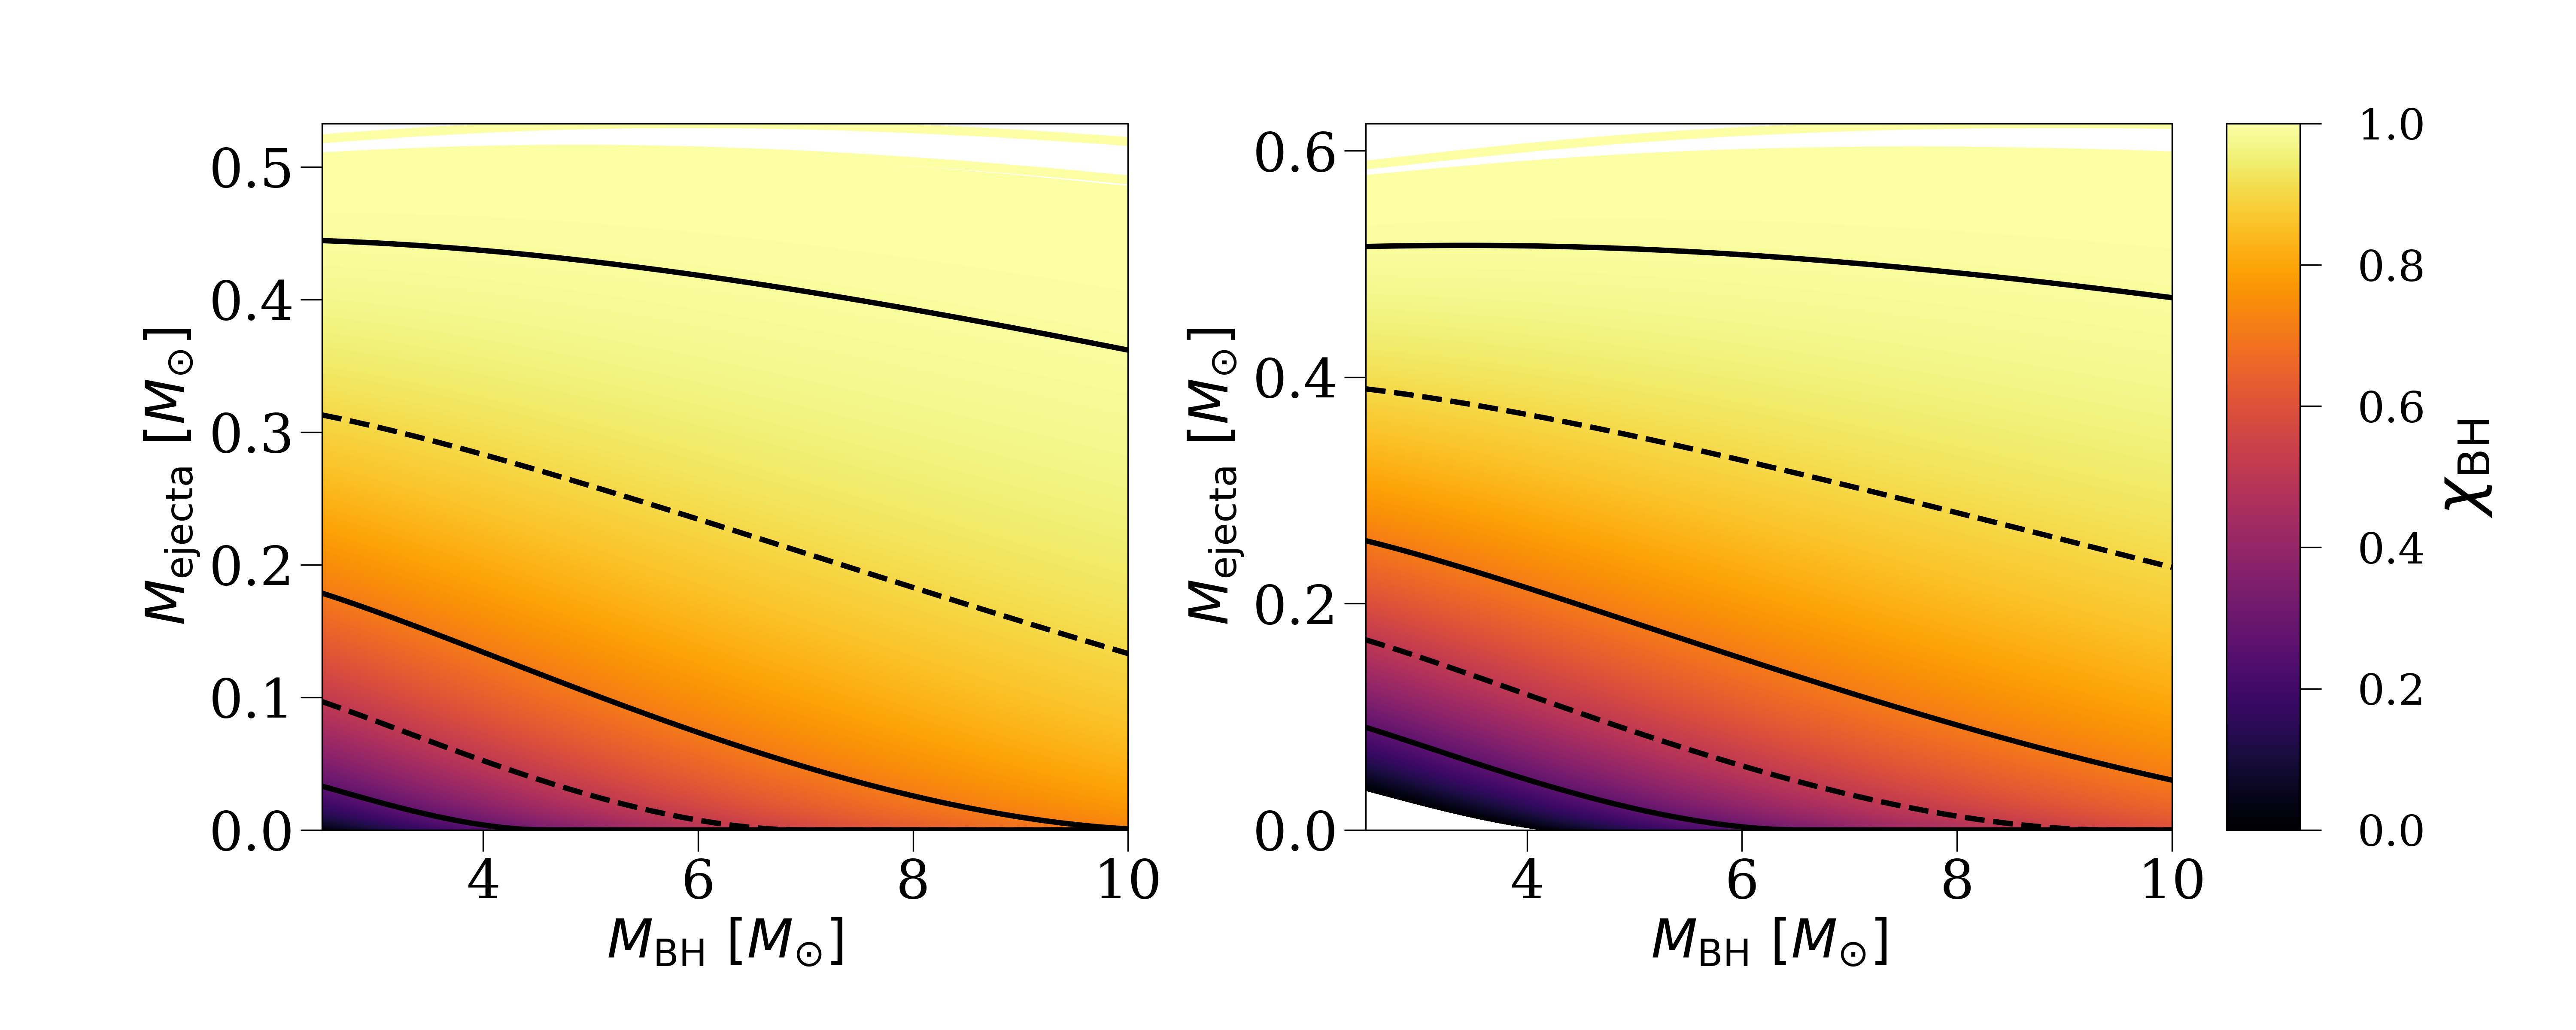
\includegraphics[width=1\textwidth]{../PlottingScripts/imagesUFDandRatios/PredictedMej.png} %CPUVsUncertaintySingleTogether.pdf}
    \caption{}
%    The number of binaries found of the target population  $N_{\mathrm{T}}$ as a function of the total number of binaries $N_{\text{binaries}}$ sampled for the traditional sampling method (gray dashed line) and the sampling method presented in this study (solid colored line). The four different panels show the simulations for each of the four target subpopulations. In each panel the duration of the exploratory phase is shown with a hashed gray area.  In the background the standard Poisson fractional uncertainties  of $0.3, 1$ and $3\%$ are shown with a dashed line.  } 
    \label{fig:PredictedMej}
\end{figure*}
%



\subsubsection{Role of BH--NS compared to NS--NS }
\begin{itemize}
	\item drake formula for rate of candidate 
\end{itemize}

\begin{equation}
	\mathcal{R}_{\rm{candidates}} \approx \mathcal{R}_{\rm{merger}} \times f_{\rm{merges \ in \ halo}} \times f_{\rm{enriches}}
\end{equation}


\section{Results}
\label{sec:result}
%

\subsection{rates of BH--NS candidates versus NS--NS candidates }
Table~\ref{tab:summary-simulations} summarizes the results from our binary population synthesis simulations focusing on the candidate systems that can enrich UFD galaxies from the different models simulated in this paper. The weight quoted in the table represent the number of candidate systems expected to form out of $10^6$ binaries drawn from the birth distributions as described in Section~\ref{sec:method}. 
The weight  of BH--NS candidates in our \Fiducial model is \fexplTwo, \EffExplTwo and   \EffRefTwo  for respectively assuming a black hole spin of $ \chi_{\rm{bh}} = 1, \chi_{\rm{bh}} = 0.5, $ and $\chi_{\rm{bh}} = 0$. 
%The first column shows the physical models simulated in this work, where we show the  the different BH--NS simulations and the results for our \Fiducial NS--NS simulation for comparison.
%The 2nd -- 4th columns show the total weight of the candidate systems in our simulation, which are defined as all the BH--NS or NS--NS mergers that merge well within a halo with mass of $M \approx 10^9 \, M_{\odot}$ $(10^8 \, M_{\odot})$, with$ r_{\rm{vir}} \approx 4.6 \rm{kpc}$ $( \approx 1.3 \rm{kpc})$ with redshift $ z = 6 $ ( $ z =  10 $). Where the different columns represent different assumptions for the spin of the black hole in the $BH--NS$ binary of $\chi_{\rm{bh}} = 1, \chi_{\rm{bh}} = 0.5, $ and $\chi_{\rm{bh}} = 0$. 
 
\begin{table*} %{Summary of Adaptive Importance Sampling method results \\}
\centering
\label{tab:comparison2}
\begin{tabular}{|l|c|c|c|c|c|c|c|}
\hline
\hline
  Model		    &   weight candidates   &   weight   candidates  		&    weight  candidates  &  weight  all    & Fraction &   $\#$ candates /   	\\
    &    $\chi_{\rm{bh}}=1$   &  $\chi_{\rm{bh}}=0.5$ 		&   $\chi_{\rm{bh}}=0$   &    &  &    $\#$ all mergers  	\\ \hline 
NS--NS \Fiducial    &  \fexplOne  & \EffExplOne  & \EffRefOne & \NxMCOne   & \NxAISOne & \gainOne  \\ \hline
BH--NS  \Fiducial   &  \fexplTwo  & \EffExplTwo  & \EffRefTwo & \NxMCTwo   & \NxAISTwo & \gainTwo  \\ %\hline
BH--NS   $Z=0.002$   &  \fexplThree  & \EffExplThree & \EffRefThree & \NxMCThree   & \NxAISThree & \gainThree  \\ %\hline
BH--NS reduced kick  &  \fexplFour  & \EffExplFour  & \EffRefFour & \NxMCFour   & \NxAISFour & \gainFour  \\
 BH--NS $\alpha =0.1$       &  \fexplFive  & \EffExplFive  & \EffRefFive & \NxMCFive   & \NxAISFive & \gainFive  \\
  BH--NS $\alpha =10$  &  \fexplSix  & \EffExplSix  & \EffRefSix & \NxMCSix   & \NxAISSix & \gainSix  \\ 
  BH--NS Fryer \texttt{RAPID}  &  \fexplSeven & \EffExplSeven  & \EffRefSeven & \NxMCSeven   & \NxAISSeven & \gainSeven  \\  
 \hline
\end{tabular}
\caption{The total weight (i.e. number) of double compact objects formed out of $10^6$ binaries simulated in each model. The total weight is derived from combining the probability of occuring of each binary in the simulation and equals `the number of binaries out of the total simulation`.  A description of the models is given in Section \ref{subsec:method-COMPASmodel}.  The 2nd to 4th column give the total weight of double compact objects that merges well within the virial radius of  a halo with mass $10^9 M_{\odot} \ (r_{\rm{vir}}   = 4.6 \, \rm{kpc})$ at $z \approx 6$. In parenthesis the total weight of the systems is shown that merge within a halo of mass   $10^8 M_{\odot} $ $ (r_{\rm{vir}}   = 1.3 \, \rm{kpc})$ at $z \approx 10$. The fifth column shows the total weight of all double compact object systems that merge within a Hubble time, and the sixth column shows the fraction  of all double compact object mergers that is a candidate system. The last column shows the total number of binaries out of $10^6$ that evolved to a candidate and to all double compact object systems.  }
\label{tab:summary-simulations}
\end{table*} 

\subsection{properties in vsys and time frame, and eccentricity versus separation frame }
%
\begin{figure*}
	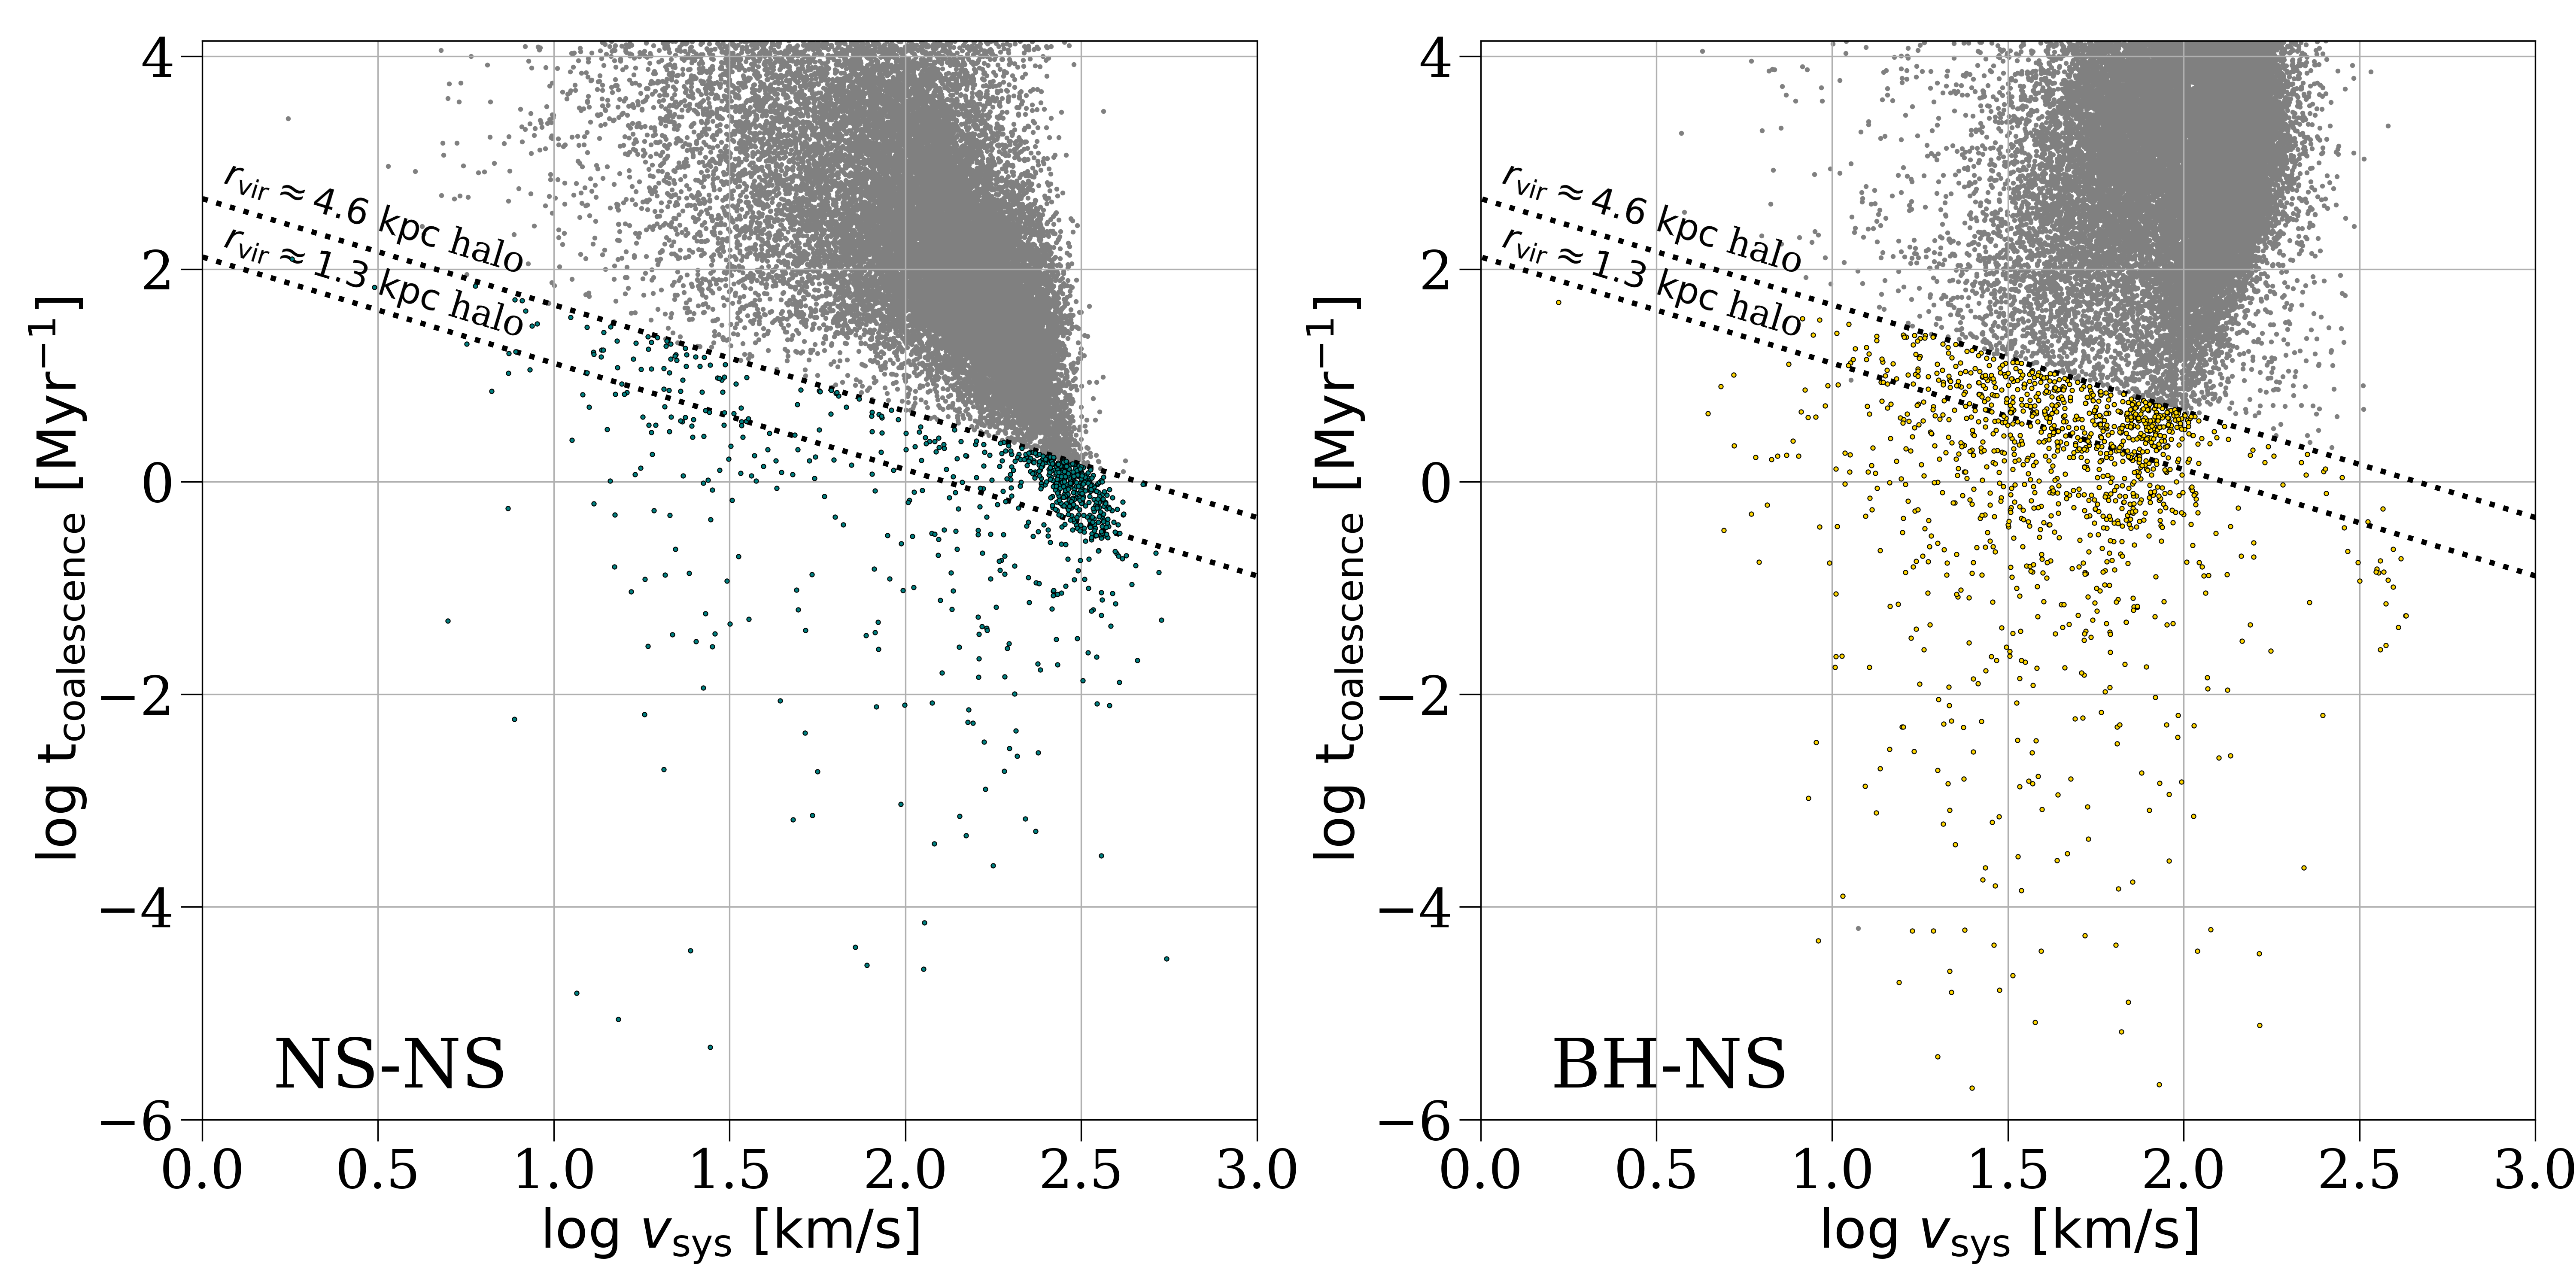
\includegraphics[width=1\textwidth]{/Users/fbro0003/Documents/git/popsynth/Papers/BroekgaardenEtAl/BHNSmergers/images/scatterCandidates_Xeff.pdf} %CPUVsUncertaintySingleTogether.pdf}
    \caption{The systematic velocity of the binary system versus the coalescence time, at the moment the double compact object formed. \textbf{[left panel:] } NS--NS mergers and candidates,   \textbf{[right panel:] } BH-NS mergers and candidate systems when assuming a high spinning BH with  $\chi_{\rm{bh}} = 0.97$. In grey all double compact object mergers of that modeled population. A small subset of those mergers, merges well within the radius of a halo of $10^9 M_{\odot} \ (r_{\rm{vir}}   = 4.6 \, \rm{kpc})$ at $z \approx 6$ or a halo of mass   $10^8 M_{\odot} $ $ (r_{\rm{vir}}   = 1.3 \, \rm{kpc})$ at $z \approx 10$.   Dotted lines indicate the maximum $v_{\rm{sys}} \times t_{\rm{coalescence}}$ that is needed to merge within those halos}
    \label{fig:NbinariesVsNHits}
\end{figure*}


%
\begin{figure*}
	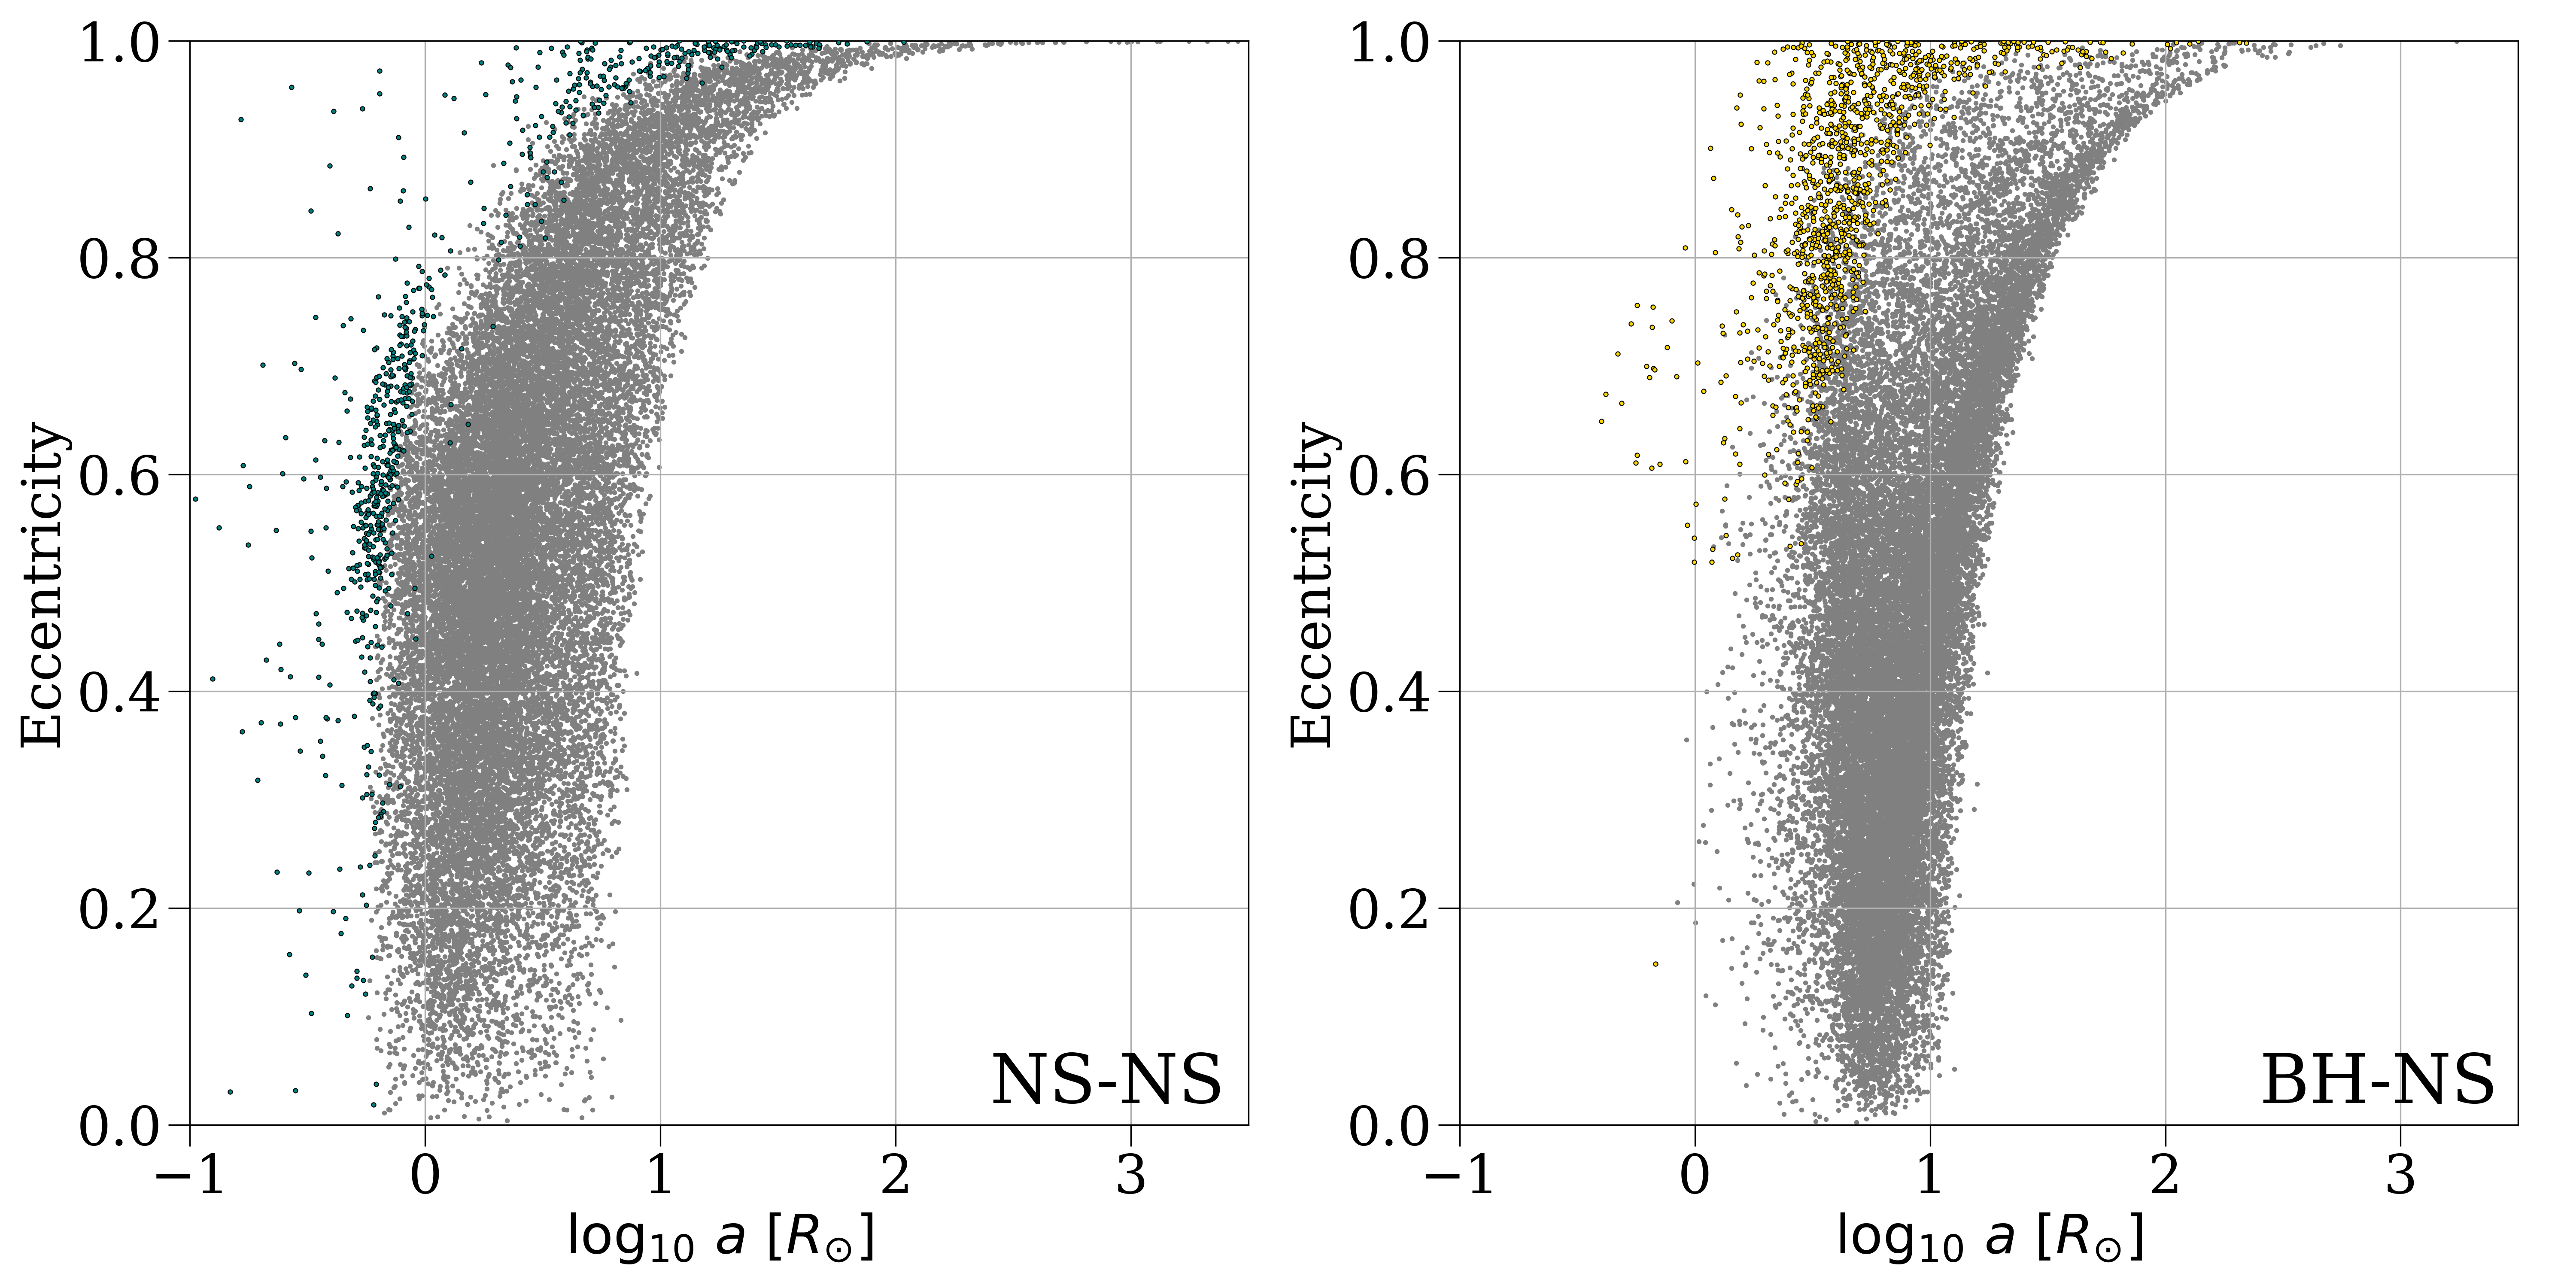
\includegraphics[width=1\textwidth]{/Users/fbro0003/Documents/git/popsynth/Papers/BroekgaardenEtAl/BHNSmergers/images/scatterCandidates_Xeff_II.pdf} %CPUVsUncertaintySingleTogether.pdf}
    \caption{The separation  of the binary system versus the eccentricity at the moment the double compact object formed. The systems that merge well within the halo of an UFD are coloured with blue or yellow.  \textbf{[left panel:] } NS--NS mergers and candidates,   \textbf{[right panel:] } BH-NS mergers and candidate systems when assuming a high spinning BH with  $\chi_{\rm{bh}} = 0.97$. In grey all double compact object mergers of that modeled population.}
    \label{fig:NbinariesVsNHits}
\end{figure*}


\subsection{properties of the candidate systems}
\begin{itemize}
	\item systematic velocities
	\item natal kick properties
	\item BH vs NS forms first  (do this here or in formation channel discussion) 
	\item traveled distance
\end{itemize}
%
\begin{figure*}
	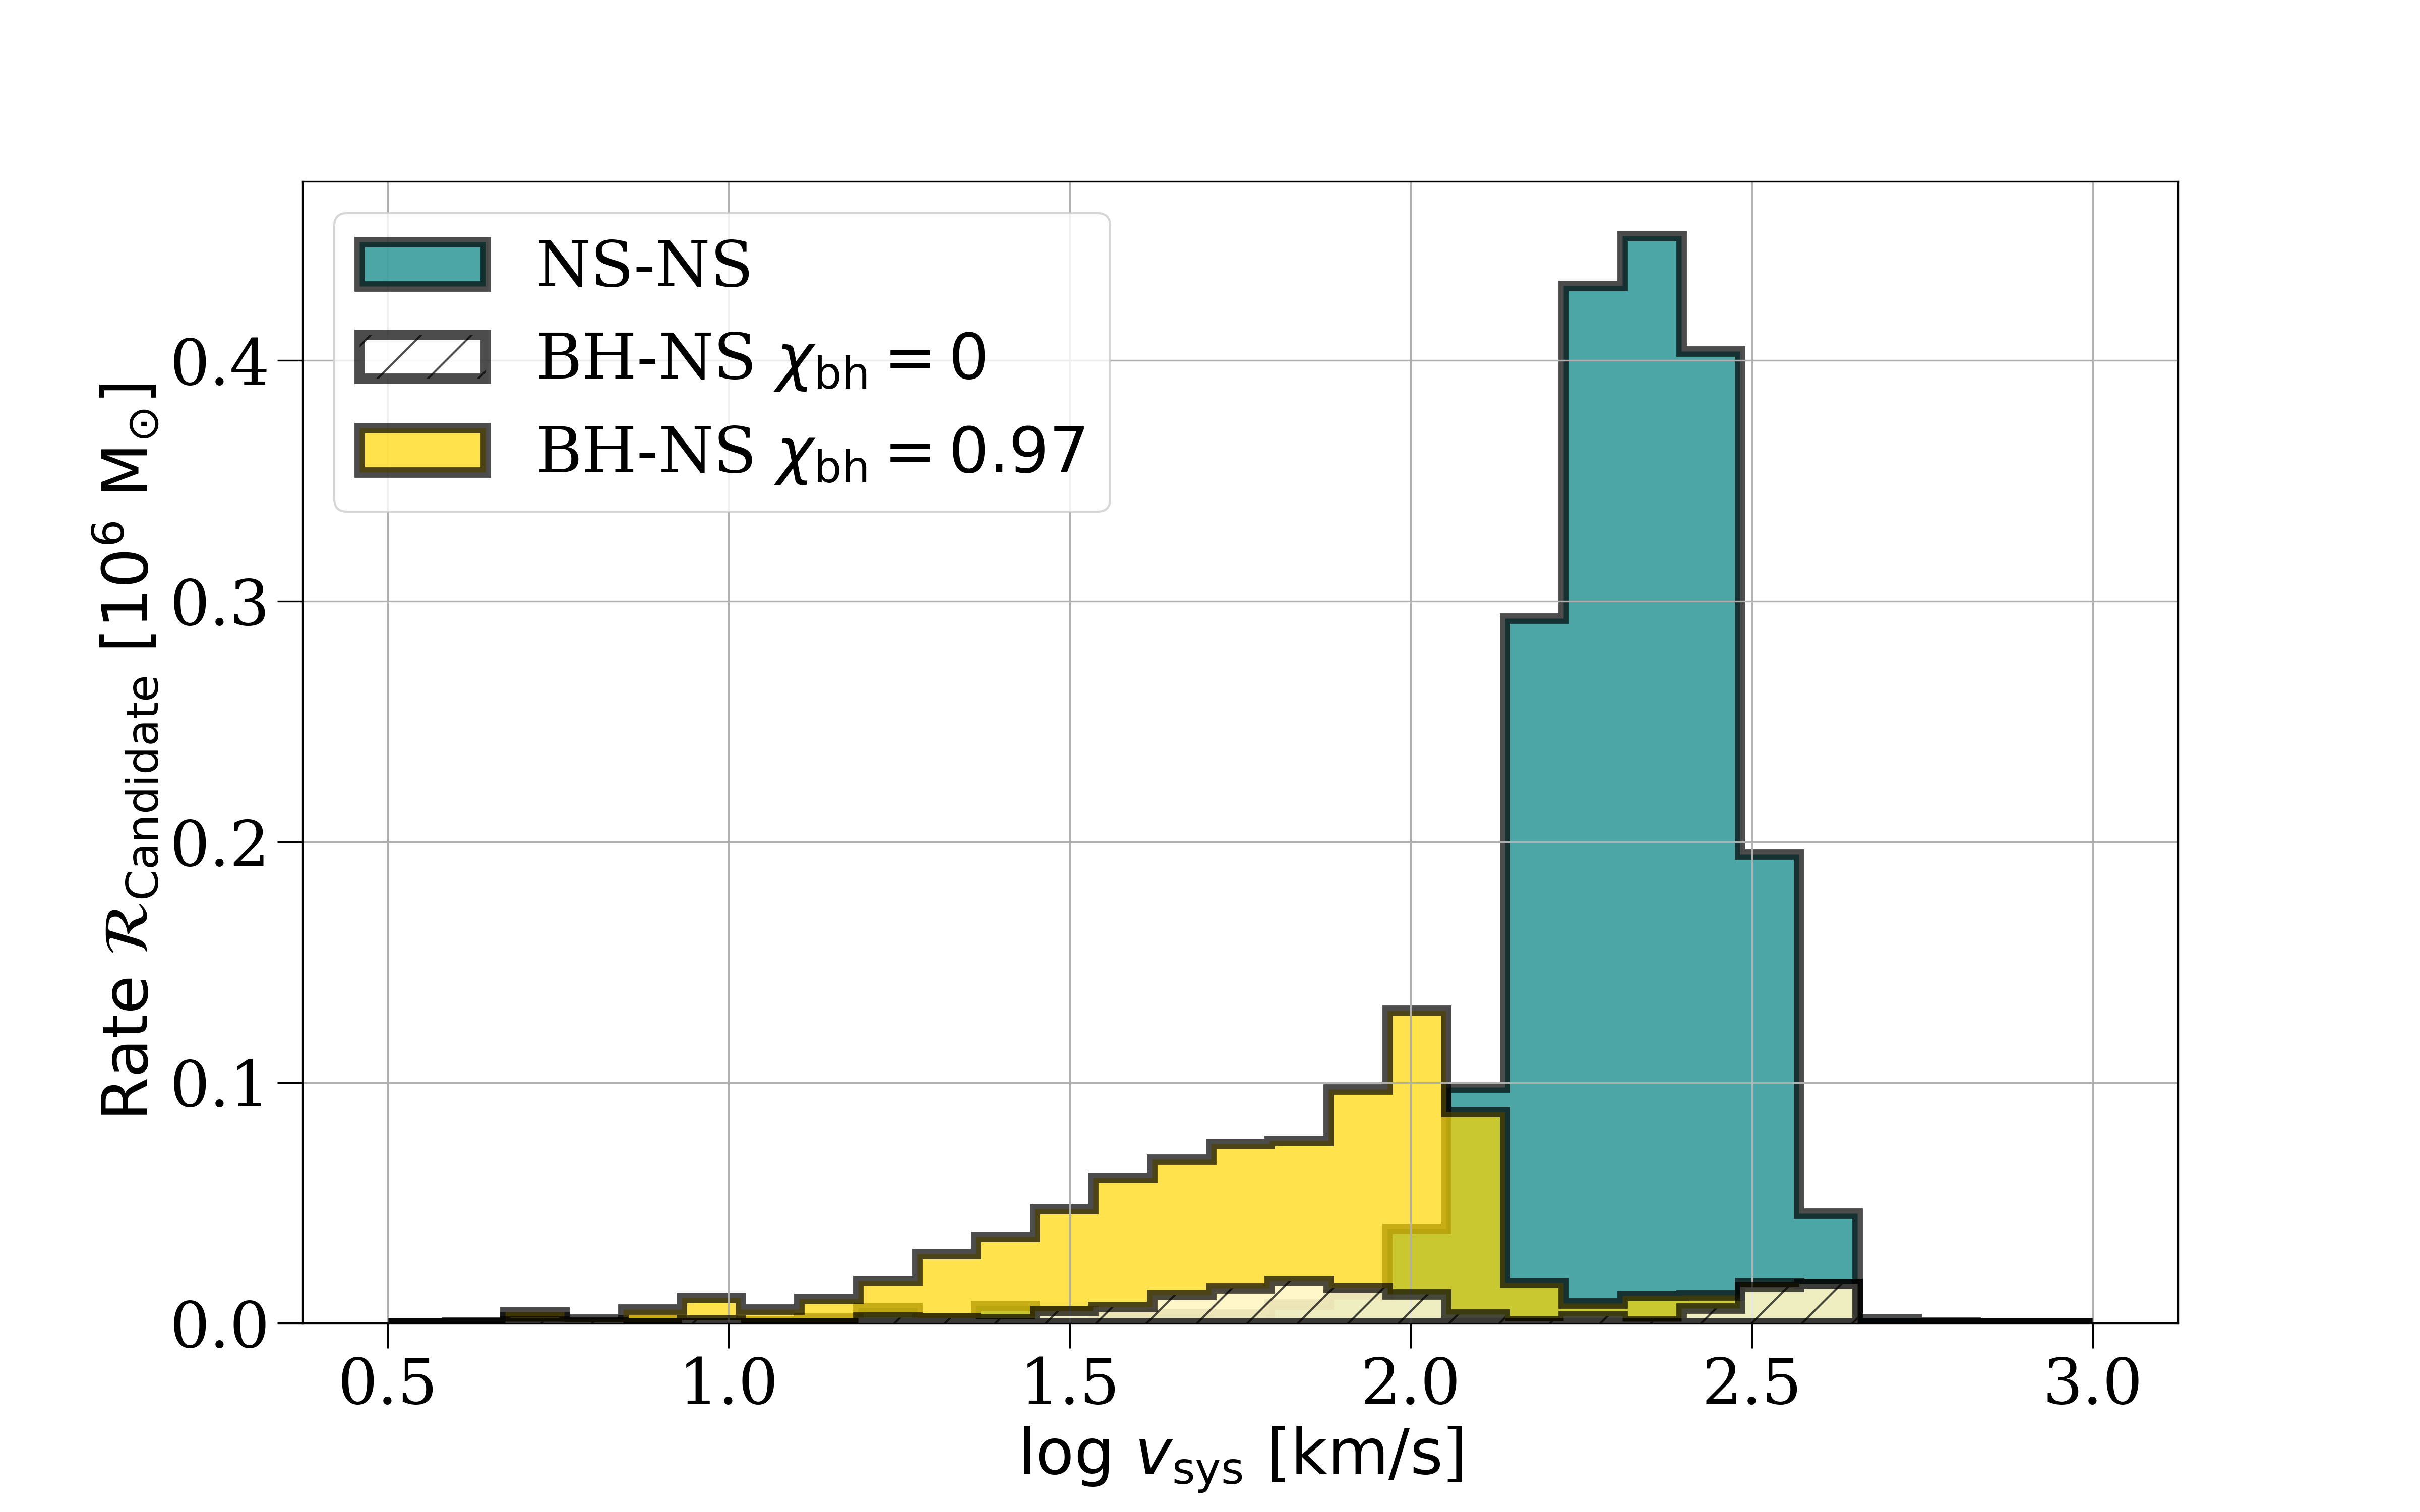
\includegraphics[width=1\columnwidth]{/Users/fbro0003/Documents/git/popsynth/Papers/BroekgaardenEtAl/BHNSmergers/images/tsystematicPDF.pdf} %CPUVsUncertaintySingleTogether.pdf}
    \caption{Distribution function of the systematic velocity of the candidate binaries after the second supernova. In blue the distribution for NS--NS candidates are shown, whereas in yellow the distribution for BH--NS systems is shown assuming a black hole spin of  $\chi_{\rm{bh}} = 0.97$ (where the hatched  area shows the distribution of BH--NS candidates if $\chi_{\rm{bh}} = 0$. It is clearly visible that NS--NS and BH--NS candidates have a distinct distribution function for $v_{\rm{sys }}$ with BH--NS having overall smaller systematic velocities}
%    The number of binaries found of the target population  $N_{\mathrm{T}}$ as a function of the total number of binaries $N_{\text{binaries}}$ sampled for the traditional sampling method (gray dashed line) and the sampling method presented in this study (solid colored line). The four different panels show the simulations for each of the four target subpopulations. In each panel the duration of the exploratory phase is shown with a hashed gray area.  In the background the standard Poisson fractional uncertainties  of $0.3, 1$ and $3\%$ are shown with a dashed line.  } 
    \label{fig:NbinariesVsNHits}
\end{figure*}
%


\begin{figure*}
	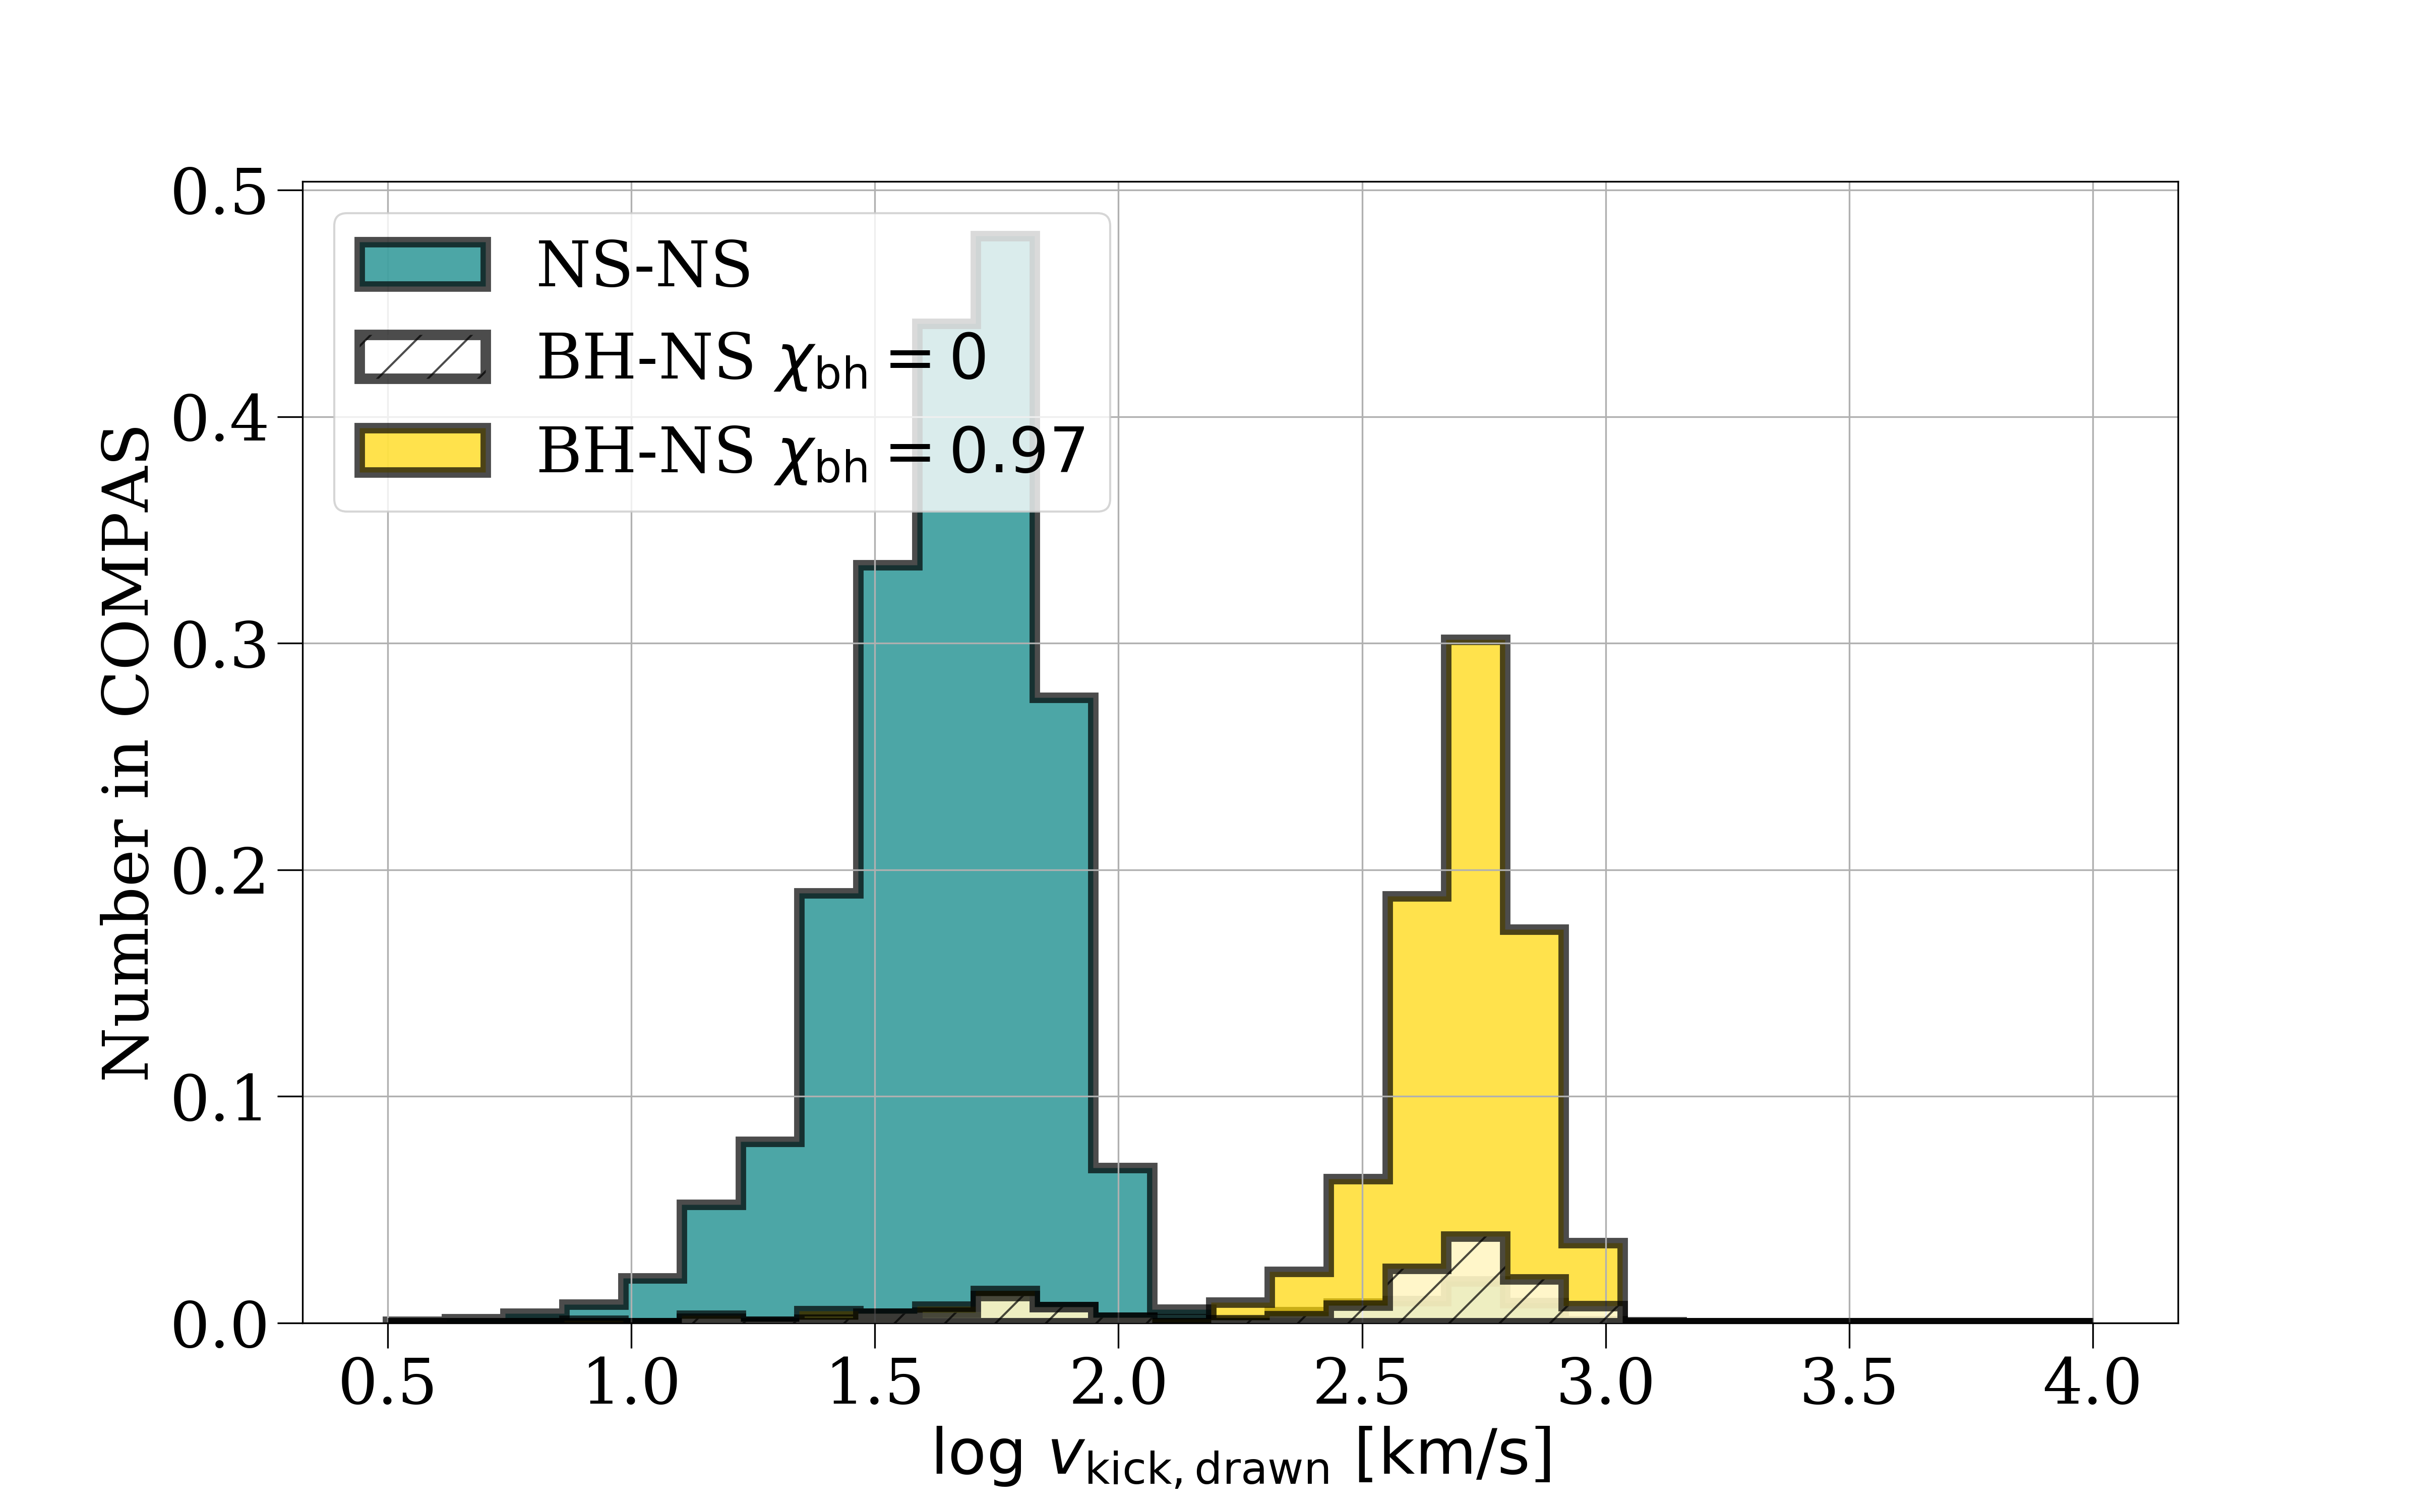
\includegraphics[width=1\columnwidth]{/Users/fbro0003/Documents/git/popsynth/Papers/BroekgaardenEtAl/BHNSmergers/images/drawnKickVelocityPDF.pdf} %CPUVsUncertaintySingleTogether.pdf}
    \caption{Distribution function of the drawn kick velocity magnitudes of the candidate binaries after the second supernova. In blue the distribution for NS--NS candidates are shown, whereas in yellow the distribution for BH--NS systems is shown assuming a black hole spin of  $\chi_{\rm{bh}} = 0.97$ (where the hatched  area shows the distribution of BH--NS candidates if $\chi_{\rm{bh}} = 0$. It is clearly visible that NS--NS and BH--NS candidates have a distinct distribution function for $v_{\rm{k }}$ with BH--NS having overall larger drawn kick velocities.}
%    The number of binaries found of the target population  $N_{\mathrm{T}}$ as a function of the total number of binaries $N_{\text{binaries}}$ sampled for the traditional sampling method (gray dashed line) and the sampling method presented in this study (solid colored line). The four different panels show the simulations for each of the four target subpopulations. In each panel the duration of the exploratory phase is shown with a hashed gray area.  In the background the standard Poisson fractional uncertainties  of $0.3, 1$ and $3\%$ are shown with a dashed line.  } 
    \label{fig:NbinariesVsNHits}
\end{figure*}
%

%
\begin{figure*}
		\includegraphics*[width=1\columnwidth]{/Users/fbro0003/Documents/git/popsynth/Papers/BroekgaardenEtAl/BHNSmergers/images/traveldistancePDF_Xeff0_97.pdf}
		\includegraphics*[width=1\columnwidth]{/Users/fbro0003/Documents/git/popsynth/Papers/BroekgaardenEtAl/BHNSmergers/images/traveldistanceCDF_Xeff0_97.pdf}
%
%    \label{fig:RateCandidateEnriching}
%\end{figure*}
%%
%%
%\begin{figure*}
		\includegraphics*[width=1\columnwidth]{/Users/fbro0003/Documents/git/popsynth/Papers/BroekgaardenEtAl/BHNSmergers/images/traveldistancePDF_Xeff0_0.pdf}
		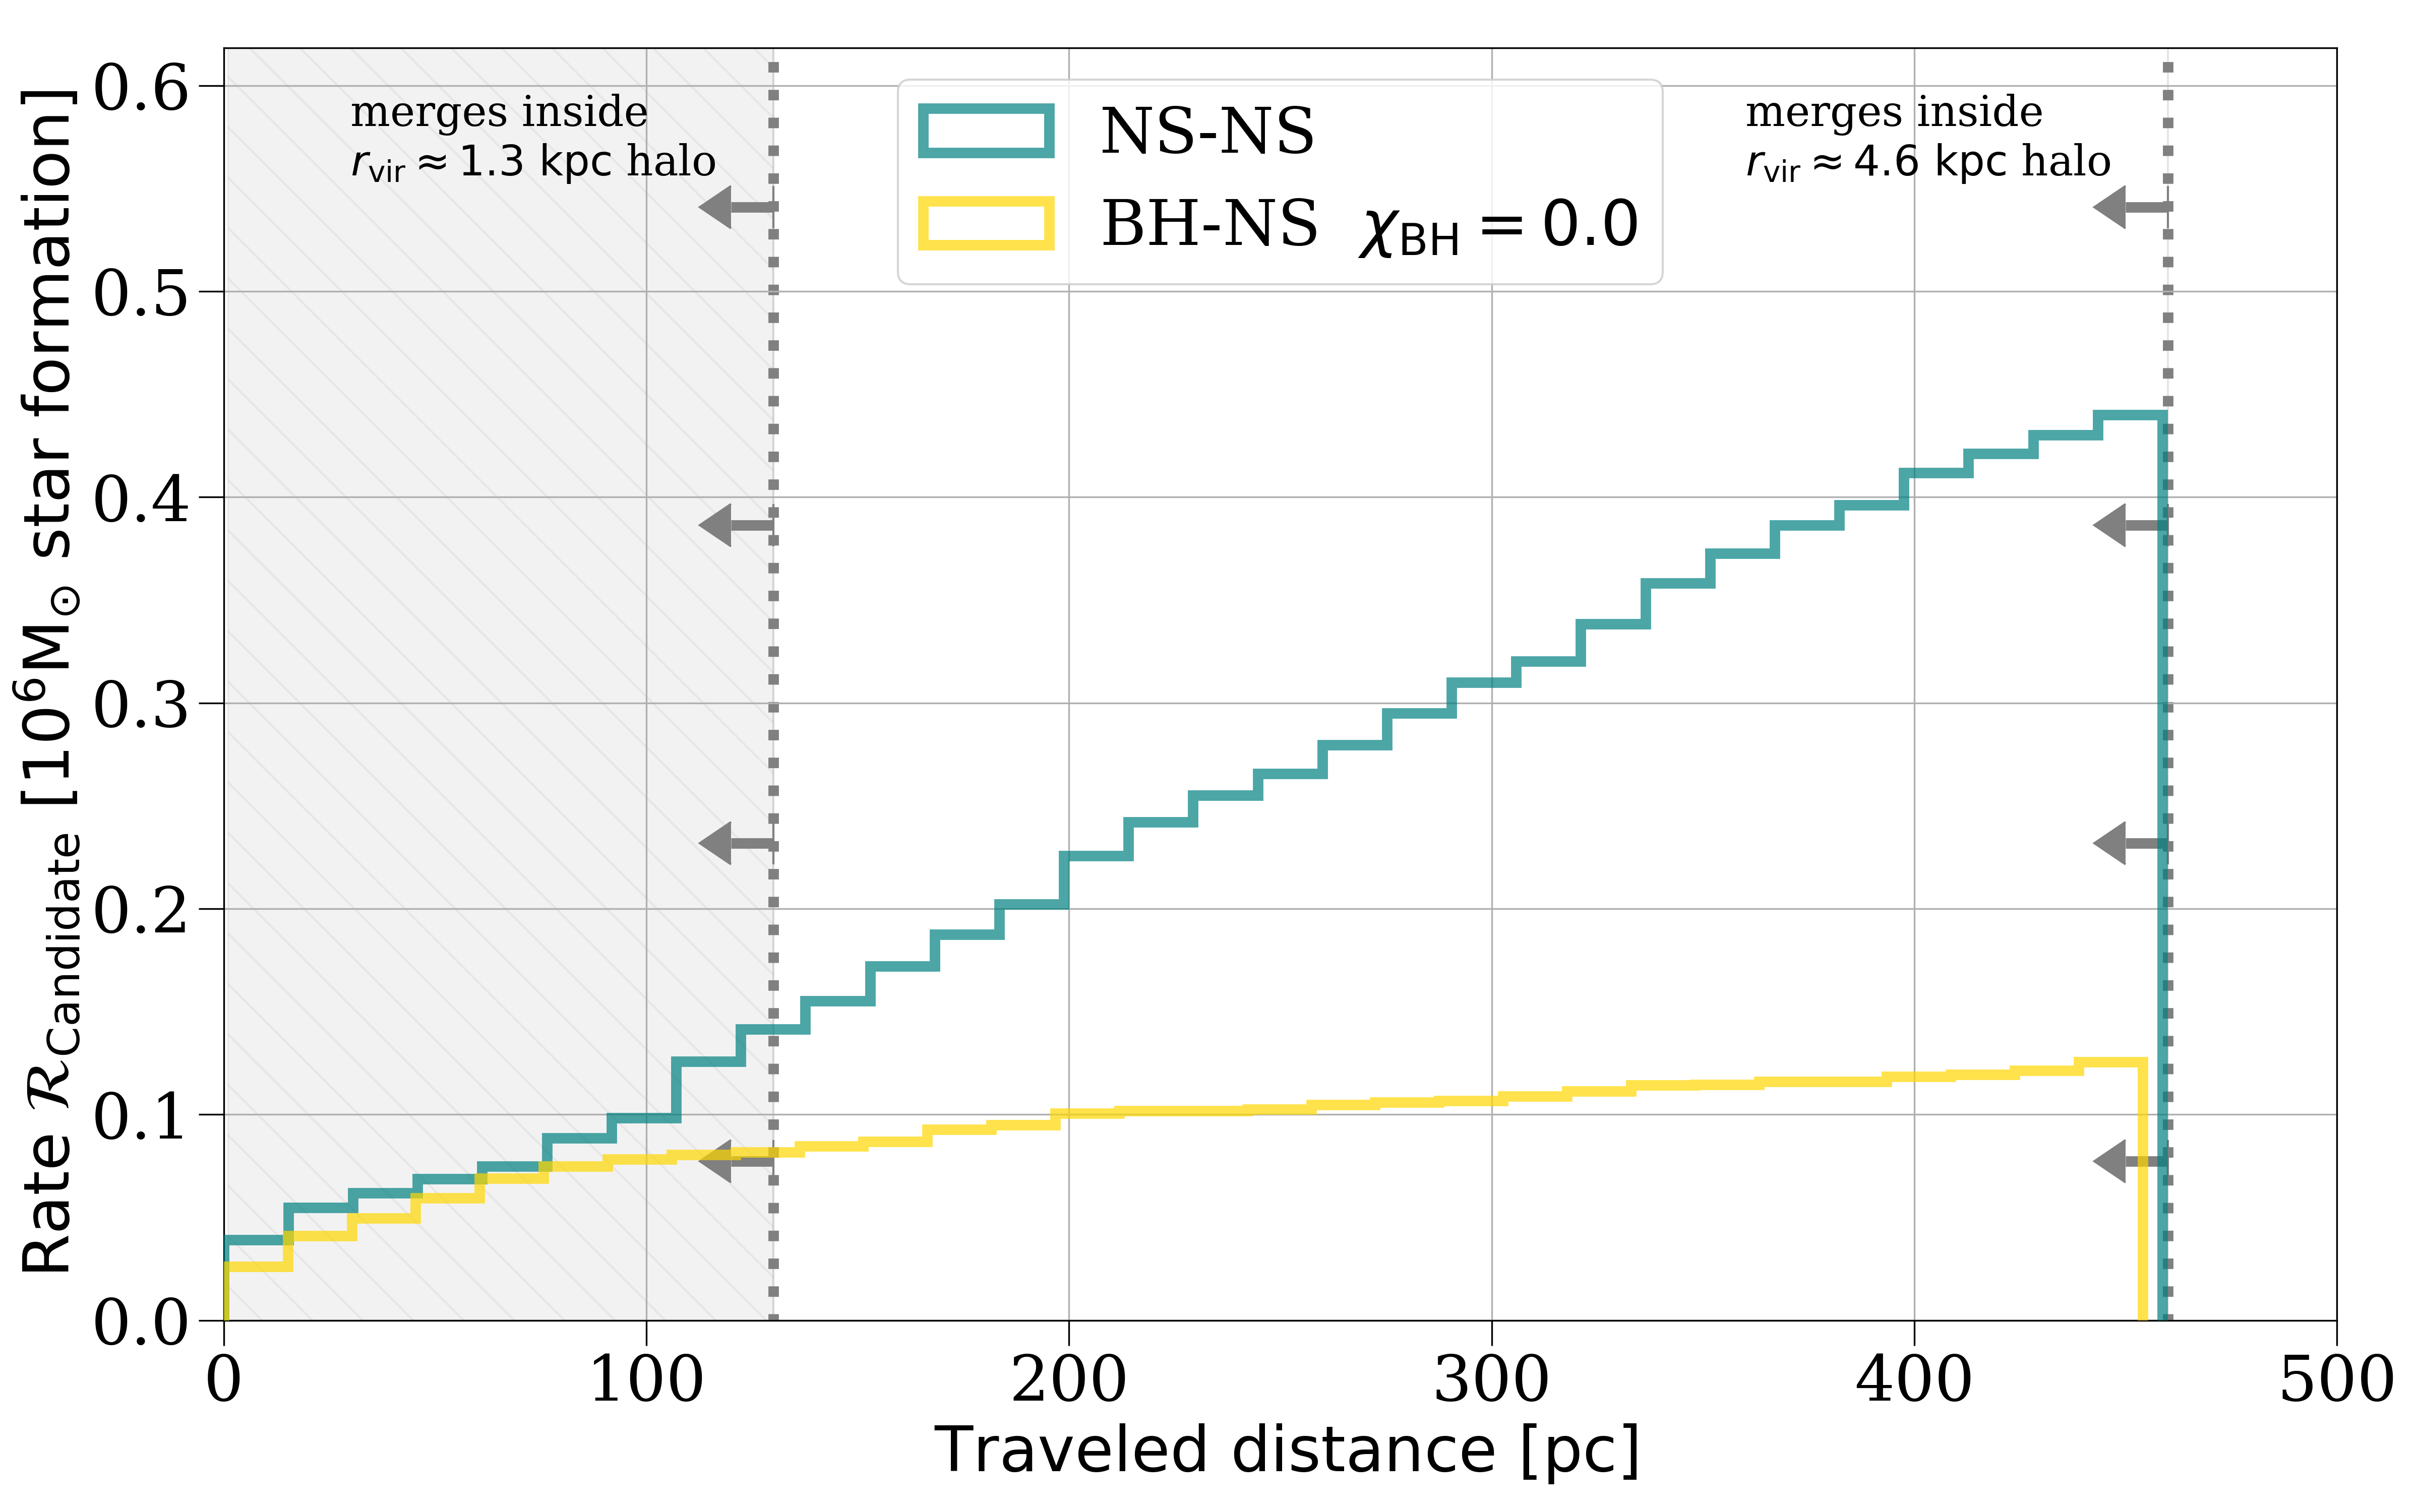
\includegraphics[width=1\columnwidth]{/Users/fbro0003/Documents/git/popsynth/Papers/BroekgaardenEtAl/BHNSmergers/images/traveldistanceCDF_Xeff0_0.pdf}
    \caption{\textbf{Left panel:} distribution function and \textbf{right panel:} cumulative distribution function of the travelled distance of the candidate binaries between the second supernova and the merger. In blue the distribution for NS--NS candidates are shown, whereas in yellow the distribution for BH--NS systems is shown. \textbf{Upper panel:}  assuming a black hole spin of  $\chi_{\rm{bh}} = 0.97$. \textbf{lower panel:} the same but now assuming BH--NS candidates have a black hole with spin $\chi_{\rm{bh}} = 0$.  BH--NS candidate rates are similar for both assumed halos if the black holes have a high spin, whereas if black holes have negligible spin, the BH--NS become mostly important for lower mass halos. } 
    \label{fig:RateCandidateEnriching}
\end{figure*}

%
\subsection{rates comparison with UFD galaxies}
%
\begin{figure*}
		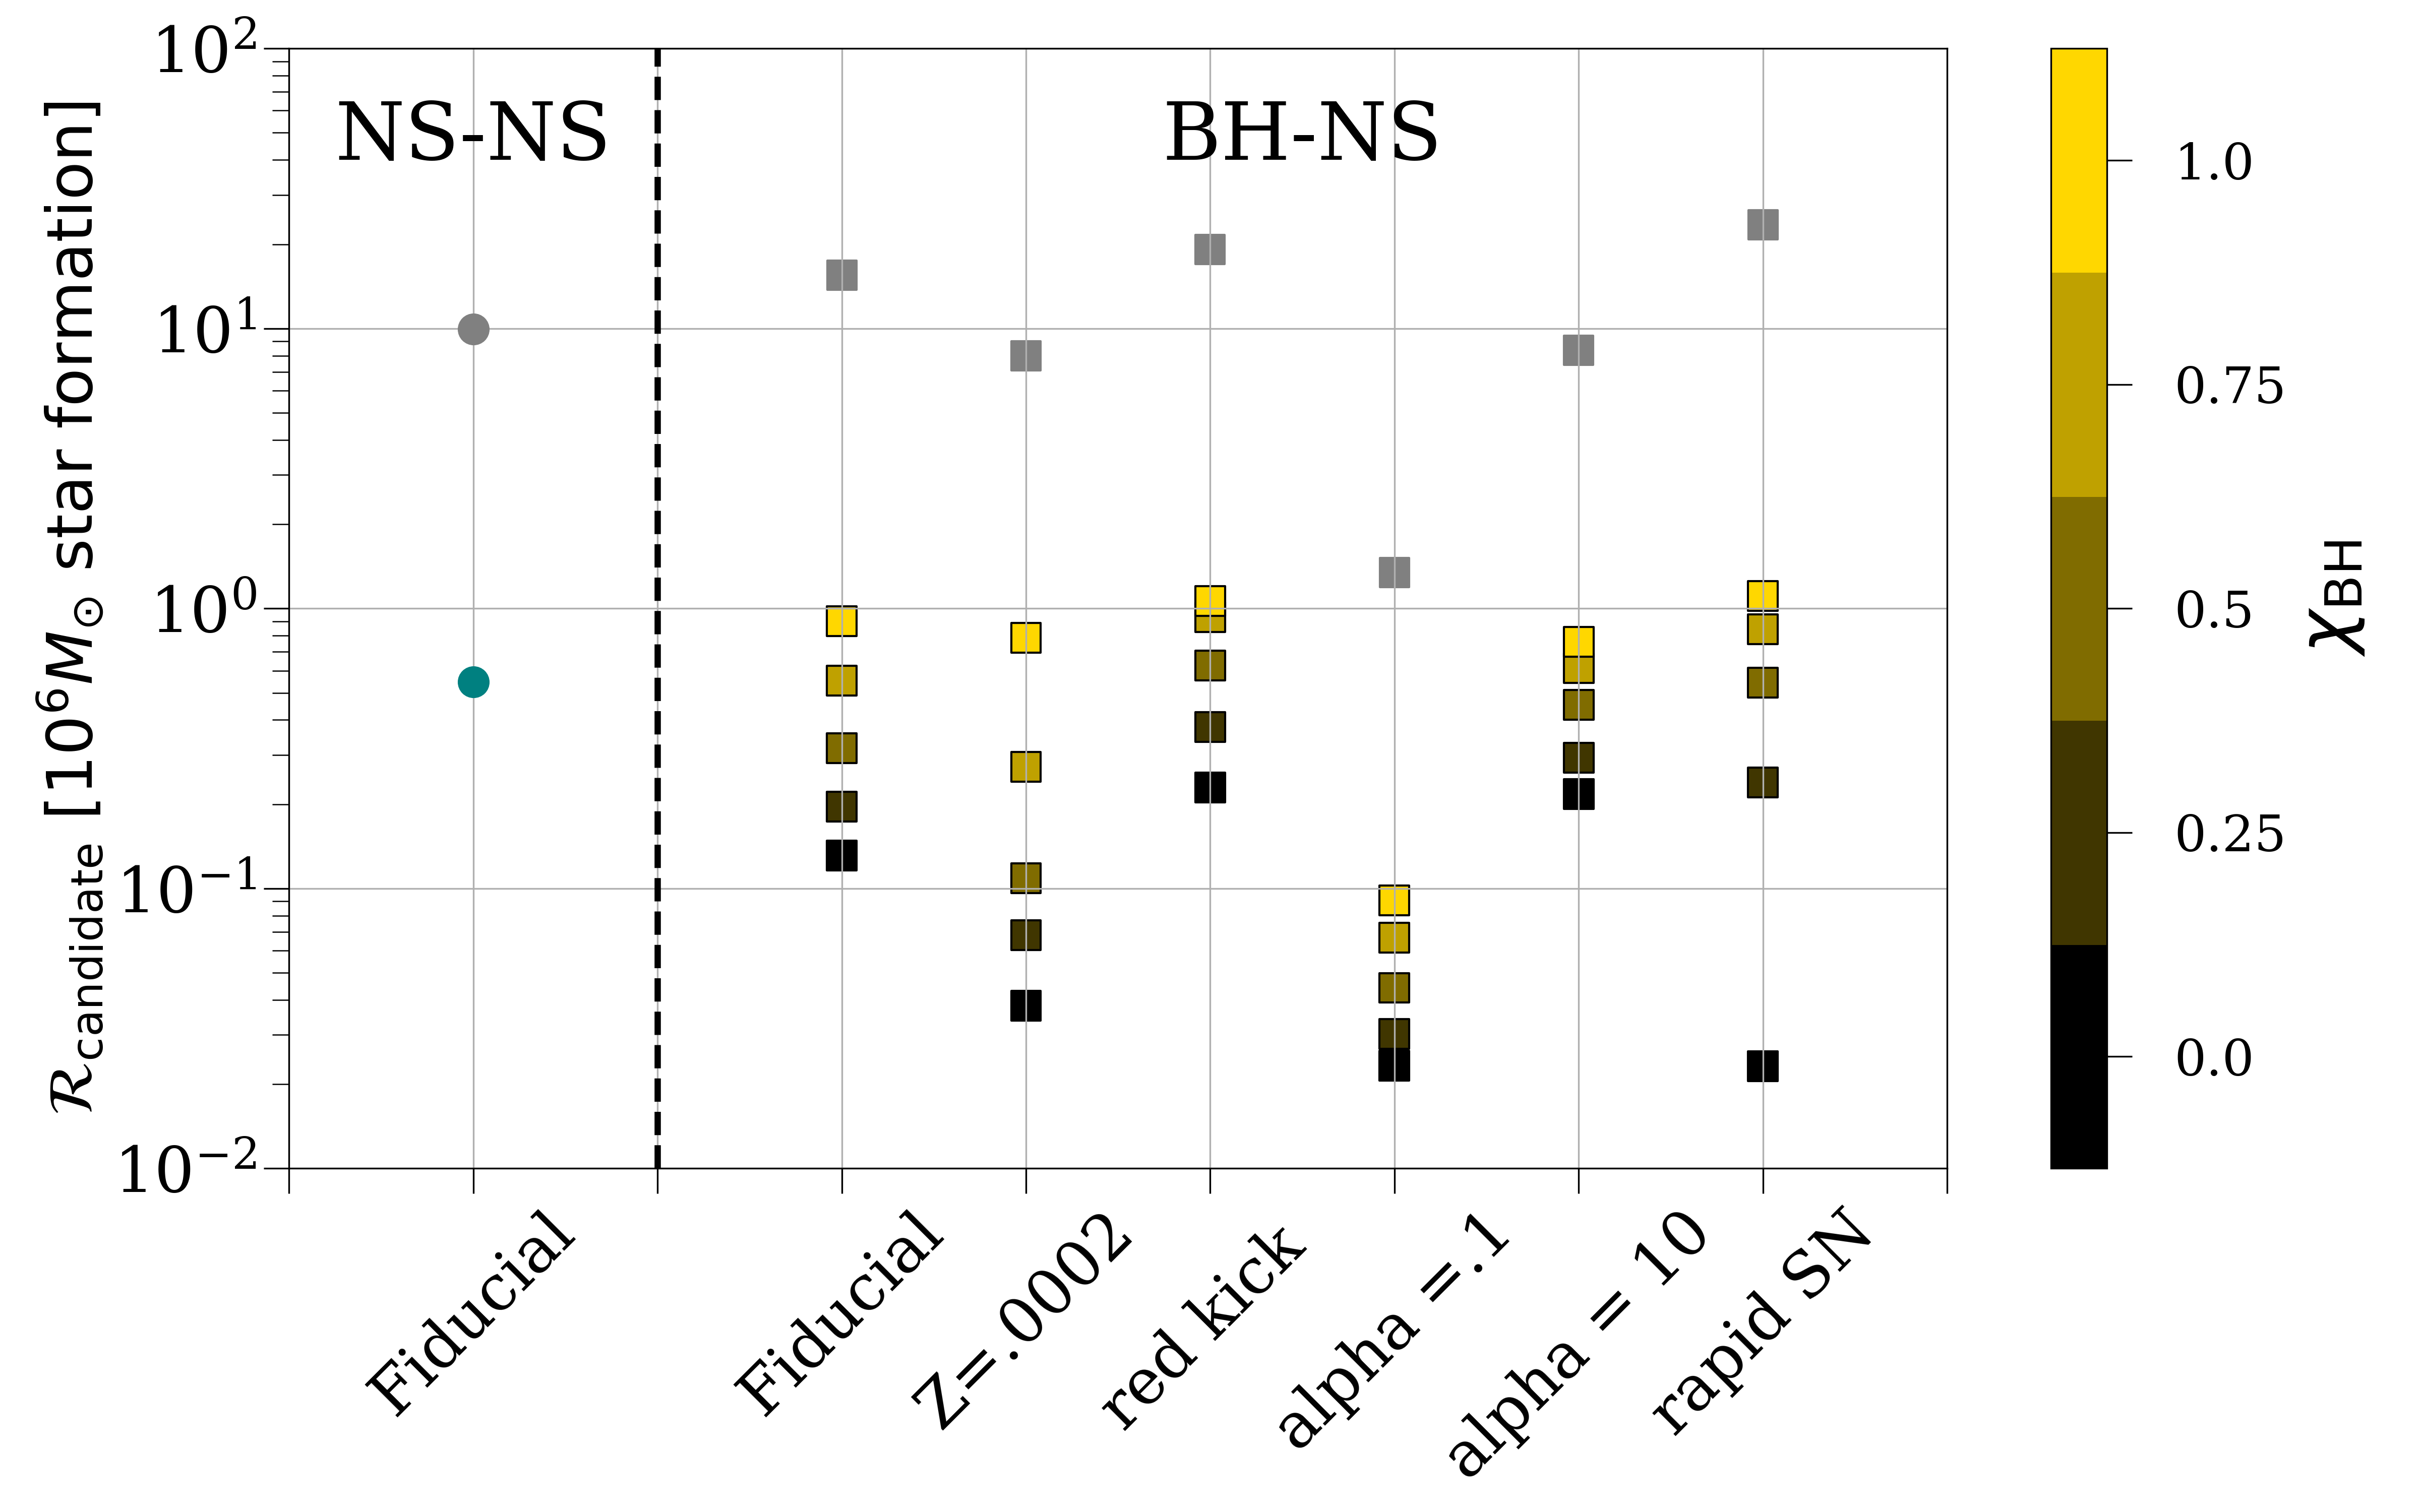
\includegraphics[width=1\textwidth]{/Users/fbro0003/Documents/git/popsynth/Papers/BroekgaardenEtAl/BHNSmergers/images/RateUFDEnrichingMergers2.pdf}
		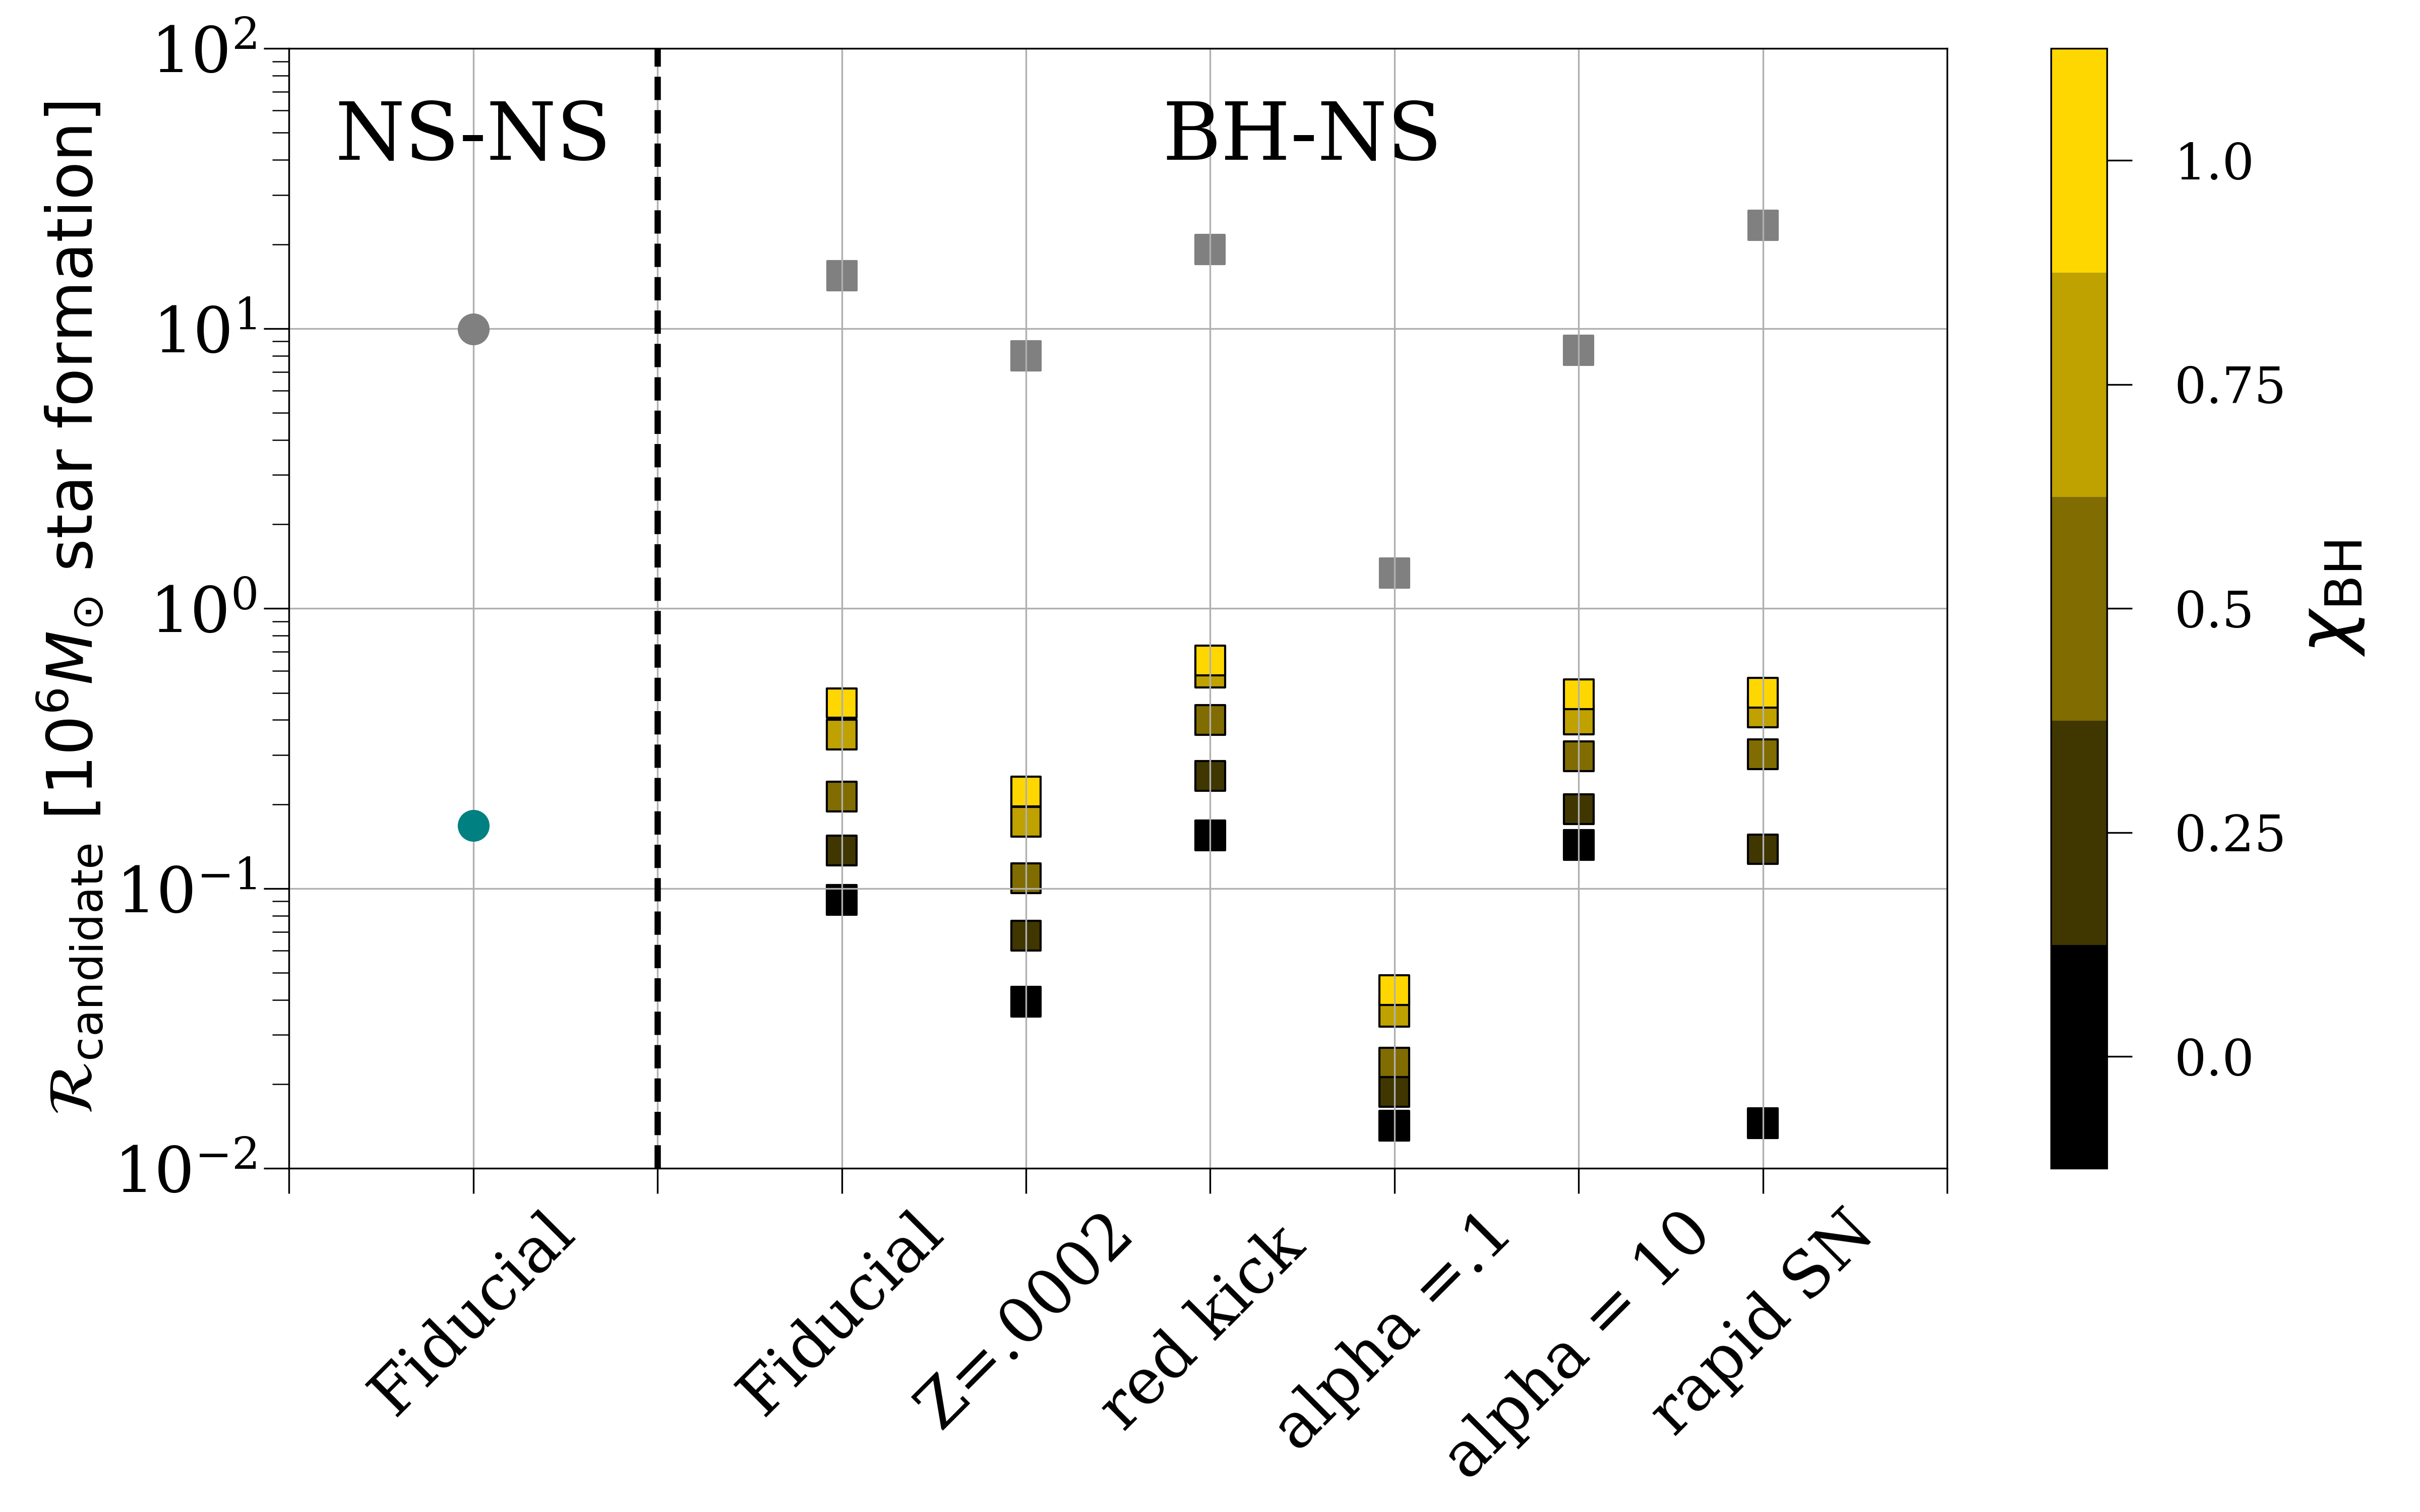
\includegraphics[width=1\textwidth]{/Users/fbro0003/Documents/git/popsynth/Papers/BroekgaardenEtAl/BHNSmergers/images/RateUFDEnrichingMergers2_Rvir1_3.pdf}
    \caption{ The formation rate of candidate  NS--NS (first cirlce data point) and BH--NS (square data points) binaries. Each data point indicates the total rate of formation of candidate systems per $10^6 \ \rm{M}_{\odot}$ star formation. There are one circle and 6 squares which correspond to the one NS--NS model and 6 BH--NS models studied here. In grey for each model the rate of all double compact mergers in a Hubble time is given. A fraction of those mergers, mergers well within the ultra-faint-dwarf galaxy, possibly makes r-processes  and merges fast enough to be able to explain the r-process enriched UFD. The rate of those candidate systems are shown with a coloured datapoint. For BH--NS candidate mergers the rate of candidate systems depends on the assumption for the black hole spin which is is shown with the colorbar} 
    \label{fig:RateCandidateEnriching}
\end{figure*}





\section{Evolutionary channels of the fast merging systems}
\label{sec:evolutionchannels}


%We find two main channels that lead to the formation of  a BH-NS merger in our \Fiducial simulation. These two main channels are illustrated in Figure \ref{fig:subchannelsMainA} and \ref{fig:subchannelsMainB}. 
%Another interesting characteristic that can be used to distinguish formation channels is whether the BH  or NS forms first. Which are hereafter referred to as respectively BH-NS and NS-BH binaries. In our \Fiducial model we find that in $60\%$
%of all systems that formed a BH-NS merger the BH was formed first. In other words, in the other $40\%$  mass transfer between the binaries causes the initially most massive star (i.e. the primary) in the binary to form the least massive compact object (namely the NS instead of the BH). This is especially
%interesting as it  has possible implications for observations. For example, it determines the fraction of  BH-NS merger progenitors that could be visible as a NS or BH X-ray binary.  Another example is that the neutron star can spin up during accretion when it is formed first. This could lead to the formation of a NS-BH binary with a millisecond pulsar \citep{Narayan:1991fn,Bethe:1998bn}. See also Section \ref{sec:discussion} for more discussion on this. 
%
%Throughout this section we distinguish three mass transfer cases: case A, B and C. These cases are characterized by the evolutionary state of the donor star when mass transfer is happening. Case A, B and C mass transfer are labels indicating that the stable mass transfer starts after the donating star is  respectively on the main sequence (case A), after hydrogen shell burning (case B) or after helium core burning (case C) \citep{1970A&A.....7..150L}. 
%
%
%
%
%
%
%
%
%\subsubsection{Channel A}
%The most common formation channel, {Channel A}, forms $88\%$ of  all BH-NS mergers in our simulation and  is the so-called \emph{classical isolated binary evolution} formation channel. This channel is characterized by a stable mass transfer phase before the first supernova explosion and a common-envelope (CE) phase after the first supernova. This channel was already suggested by \citet{smarr1976binary} to produce compact object mergers, but has since been widely studied and thought to produce double compact object mergers (e.g. \citealt{bethe1998evolution, voss2003galactic, postnov2014evolution, tauris2017formation, mandel2018merging} and references therein).   
%
%
%
%
%In  this formation channel the BH is formed first in $61\%$ of the cases whilst in the other $39\%$ of the cases the primary star forms the NS. 
% In this channel, the binary undergoes the following steps:
%% 
%
%
%\begin{enumerate}
%	\item two massive stars (of spectral type O or B) are born in a binary system with $10 < M_1 / M_{\odot} < 70$ ,   $10 < M_2 / M_{\odot} < 45$ and  $0.1 < a_i / \mathrm{[AU]} < 15 $. 
%	\item at a critical point, the primary star $M_1$ reaches the end of its main sequence and starts expanding. The star fills its Roche-lobe and starts  case A or case B mass transfer through stable Roche-lobe overflow (RLO) donating its hydrogen rich envelope to the secondary star that can accrete substantially. This leaves the primary as a helium star which can be observed as a Wolf-Rayet star (see e.g. \citealt{crowther2007physical,langer1994towards}). Especially early case B mass transfer occurs on small timescales set by the thermal timescale making it often the case that the secondary cannot accrete at the same rate as the mass is donated leading to nonconservative mass transfer. Case A mass transfer usually occurs on nuclear timescales which are much longer which gives the secondary more time to substantially accrete mass. These systems can therefore more often form a NS-BH system.   
%		%
%\begin{figure}
%\begin{center}
%\Large {\textbf{\hspace{-1cm}Channel A }}\par\medskip
%	\includegraphics[width=0.8\columnwidth]{/Users/fbro0003/Documents/git/popsynth/Papers/BroekgaardenEtAl/BHNSmergers/images/ChannelANoLabel.pdf}
%    \caption{Schematic view of formation channel
%A leading to a BH-NS or NS-BH merger in a Hubble time. This
%formation channel is characterized by a single-core common-envelope phase. }
%    \label{fig:subchannelsMainA}
%\end{center}
%\end{figure}
%%
%	\item eventually the primary star is at the end of its life and  can undergo after several wind-driven mass loss phases (e.g. LBV phases) a supernova explosion leaving behind a BH  or NS   in respectively ($61\%$) or ($39\%$) of the BH-NS merger cases. Which compact object type is formed is determined in COMPAS based on the mass of the C/O core.   Instead, the system can also disrupt due to, e.g., the Blaauw kick or natal kick that can be imparted during the supernova \citep{1961BAN....15..265B,1998A&A...330.1047T}. 
%	\item later on the secondary star can also  expand as it reaches the end of its MS and fill its Roche lobe. Due to the extreme mass ratio between the two stars in the binary system in combination with the mass accepting star being a compact object that can only accrete a very small fraction of the donated mass due to the accretion being Eddington lmimited, the mass transfer is highly non-conservative. This results in a substantial removal of angular momentum from the binary through the non-conservative mass loss which drastically shrinks the separation of the binary. This leads the binary in a so-called common envelope evolution phase that drastically  shrinks the separation of the system as orbital energy is converted to heat up the envelope.
%	\item If enough energy is injected into the envelope it can be successfully ejected and the binary system survives in a smaller orbit. If this is not the case the binary could instead merge.  
%	\item eventually, the secondary can also undergo a supernova explosion leaving behind a NS $(61 \%)$ or BH $(39 \%)$ as the compact remnant. 
%	\item the binaries will spiral in under the loss of orbital energy due to gravitational waves. If the separation is small enough this inspiral can lead to a merger within a Hubble time that then produces the gravitational waves that we can observe today. 
%\end{enumerate}
%
%Moreover, some of the systems undergoing channel A also have a stable mass transfer phase in between the common-envelope phase and the second supernova, which is not depicted in Figure~\ref{fig:subchannelsMainA}. 
%See also Appendix \ref{app-detailedEvolution}  and Figure \ref{fig:app-initial_ChannelABH} and \ref{fig:app-initial_ChannelANS} therein for the detailed evolution of examples of binary systems undergoing formation channel A.  \\
%
%
%
%
%
%\subsubsection{Channel B}
%
%The second most dominant formation channel, channel B, leading to a BH-NS merger in a Hubble time is characterized by the binary initiating a so-called double-core common-envelope phase. This is a phase similar to the single-core common-envelope phase (see Section 2.2.4) during which both stars have evolved from the main sequence and consist of a prominent core-envelope structure when the primary initiates unstable Roche-lobe mass transfer (see e.g. \citealt{1995ApJ...440..270B,Belczynski:2000wr, Dewi:2006bx}). In such a case, both envelopes are a prominant part of the common envelope and as a result the shared envelope is often more massive than average. This occurs commonly when the first mass transfer phase is unstable in case of Case C mass transfer. The progenitors of this channel are especially binaries  which have initially equal masses. This channel forms $5.5\%$ of all the BH-NS mergers from the \Fiducial model. 
% In   $70\%$ of the cases of channel B the BH forms first whilst in the other $30\%$ of the cases the NS forms first.  
%See also Appendix \ref{app-detailedEvolution}  and Figure \ref{fig:app-initial_ChannelBBH} and \ref{fig:app-initial_ChannelBNS} therein for the detailed evolution of examples of binary systems undergoing formation channel A.  \\
%
%
%
%
% 
% %
%
%\begin{figure}
%\begin{center}
%\Large {\textbf{\hspace{-0.5cm}Channel B }}\par\medskip
%	\includegraphics[width=0.8\columnwidth]{/Users/fbro0003/Documents/git/popsynth/Papers/BroekgaardenEtAl/BHNSmergers/images/ChannelBNoLabel.pdf}
%    \caption{Schematic view of formation channel B leading to a
%BH-NS or NS-BH merger in a Hubble time. This channel is char-
%acterised by a double core common-envelope phase.}
%    \label{fig:subchannelsMainB}
%\end{center}
%\end{figure}
%% 
%

 
 

\section{Discussion}
\label{sec:discussion}
%
\begin{itemize}
	\item discussion on observations on spins of black holes (LIGO vs X-ray binaries) 
	\item discussion on theory of spins of black holes (e.g. Tassos Fragos ) 
	\item other possible model variations
	\item BH-NS pulsar systems...
	\item these results can also be important for BH--NS as sGRB progenitors 
	\item yields of r-process elements NS--BH vs NS--NS 
\end{itemize}


\section{Conclusions}
\label{sec:conclusion}













\section*{Acknowledgements}

 

FSB thanks the the Kavli Foundation, Niels Bohr institute and DARK Cosmology Centre in Copenhagen for their hospitality and for organizing the Kavli summer school in gravitational-wave astrophysics 2017.  FSB was supported by the HPC  Europa3 grant, McKinsey grant and Kapteyn grant..




%%%%%%%%%%%%%%%%%%%%%%%%%%%%%%%%%%%%%%%%%%%%%%%%%%

%%%%%%%%%%%%%%%%%%%% REFERENCES %%%%%%%%%%%%%%%%%%

% The best way to enter references is to use BibTeX:

\bibliographystyle{mnras}
\bibliography{my_bib} % if your bibtex file is called example.bib


% Alternatively you could enter them by hand, like this:
% This method is tedious and prone to error if you have lots of references
%\begin{thebibliography}{99}
%\bibitem[\protect\citeauthoryear{Author}{2012}]{Author2012}
%Author A.~N., 2013, Journal of Improbable Astronomy, 1, 1
%\bibitem[\protect\citeauthoryear{Others}{2013}]{Others2013}
%Others S., 2012, Journal of Interesting Stuff, 17, 198
%\end{thebibliography}

%%%%%%%%%%%%%%%%%%%%%%%%%%%%%%%%%%%%%%%%%%%%%%%%%%

%%%%%%%%%%%%%%%%% APPENDICES %%%%%%%%%%%%%%%%%%%%%

\appendix



%





 %%%%%%%%%%%%%%%%%%%%%%%%%%%%%%%%%%%%%%%%%%%%%%%%%%


% Don't change these lines
\bsp	% typesetting comment
\label{lastpage}
\end{document}

% End of mnras_template.tex



